\documentclass[9pt, landscape]{extarticle}
\usepackage{ctex}
\usepackage{multicol}
\usepackage{calc}
\usepackage{ifthen}
\usepackage[landscape]{geometry}
\usepackage{hyperref}
\usepackage{lipsum}
\usepackage{amsmath}
\usepackage{amssymb}
\usepackage[cal=boondoxo]{mathalpha}
\usepackage{graphicx}
\usepackage{float}
\usepackage{wrapfig}
\usepackage{xcolor}
\usepackage{setspace}
\usepackage{array}
\usepackage{subcaption}


\numberwithin{equation}{section}


% To make this come out properly in landscape mode, do one of the following
% 1.
%  pdflatex latexsheet.tex
%
% 2.
%  latex latexsheet.tex
%  dvips -P pdf  -t landscape latexsheet.dvi
%  ps2pdf latexsheet.ps


% If you're reading this, be prepared for confusion.  Making this was
% a learning experience for me, and it shows.  Much of the placement
% was hacked in; if you make it better, let me know...


% 2008-04
% Changed page margin code to use the geometry package. Also added code for
% conditional page margins, depending on paper size. Thanks to Uwe Ziegenhagen
% for the suggestions.

% 2006-08
% Made changes based on suggestions from Gene Cooperman. <gene at ccs.neu.edu>


% To Do:
% \listoffigures \listoftables
% \setcounter{secnumdepth}{0}


% This sets page margins to .5 inch if using letter paper, and to 1cm
% if using A4 paper. (This probably isn't strictly necessary.)
% If using another size paper, use default 1cm margins.
\ifthenelse{\lengthtest { \paperwidth = 11in}}
	{ \geometry{top=.2in,left=.2in,right=.2in,bottom=.2in} }
	{\ifthenelse{ \lengthtest{ \paperwidth = 297mm}}
		{\geometry{top=1cm,left=1cm,right=1cm,bottom=1cm} }
		{\geometry{top=1cm,left=1cm,right=1cm,bottom=1cm} }
	}

% Turn off header and footer
\pagestyle{empty}
 

% Redefine section commands to use less space
\makeatletter
\renewcommand{\section}{\@startsection{section}{1}{0mm}%
                                {-1ex plus -.5ex minus -.2ex}%
                                {0.5ex plus .2ex}%x
                                {\normalfont\large\bfseries}}
\renewcommand{\subsection}{\@startsection{subsection}{2}{0mm}%
                                {-1explus -.5ex minus -.2ex}%
                                {0.5ex plus .2ex}%
                                {\normalfont\normalsize\bfseries}}
\renewcommand{\subsubsection}{\@startsection{subsubsection}{3}{0mm}%
                                {-1ex plus -.5ex minus -.2ex}%
                                {1ex plus .2ex}%
                                {\normalfont\small\bfseries}}
\makeatother

% Define BibTeX command
\def\BibTeX{{\rm B\kern-.05em{\sc i\kern-.025em b}\kern-.08em
    T\kern-.1667em\lower.7ex\hbox{E}\kern-.125emX}}

% Don't print section numbers
% \setcounter{secnumdepth}{0}
\setlength{\parskip}{0em}


% \setlength{\parindent}{0pt}
% \setlength{\parskip}{0pt plus 0.5ex}


\newcommand{\dd}{\mathrm{d}}
\newcommand{\pp}{\partial}


% -----------------------------------------------------------------------

\begin{document}

\setstretch{1.0}

\raggedright
\footnotesize
\begin{multicols}{3}

\section{导论}
\section{燃烧与热化学}
\subsection{概述}
\subsection{热力学参数关系式回顾}
\subsubsection{广延量和强度量}
\textbf{广延量:}取决于物质的数量(质量或物质的量),一般大写;{\textbf{强度量:}单位质量(或物质的量)来表示},数值与物质的量无关。\textit{单位物质的量的在本书中会加上划线},如$\overline{u}$,单位质量的则不加划线,如$u$。

\subsubsection{状态方程}
\begin{eqnarray}
    PV&=&nR_uT\\
    PV&=&mRT\\
    Pv&=&RT\\
    P&=&\rho RT
\end{eqnarray}
$R_u=8315~\mathrm{J/(kmol\cdot K)}$, $R=R_u/\mathrm{MW}$, $\rho=1/v=m/V$.

\subsubsection{状态热方程}
\begin{multicols}{2}
    \tiny
    \begin{eqnarray*}
        u&=&u(T,v)\\
        h&=&h(T, P)
    \end{eqnarray*}
    \begin{eqnarray*}
        \mathrm{d}u&=&\left({\frac{\partial u}{\partial T}}\right)_{v}\mathrm{d}T+\left({\frac{\partial u}{\partial v}}\right)_{T}\mathrm{d}v\\ 
        \mathrm{d}h&=&\left({\frac{\partial h}{\partial T}}\right)_{p}\mathrm{d}T+\left({\frac{\partial h}{\partial P}}\right)_{T}\mathrm{d}P
    \end{eqnarray*}
    \begin{eqnarray*}
        c_{v}&\equiv&\left(\frac{\partial u}{\partial T}\right)_{v}\\
    c_{p}&\equiv&\left({\frac{\partial h}{\partial T}}\right)_{P}
    \end{eqnarray*}
    
    对于理想气体,$(\partial u/\partial v)_T$和$(\partial h/\partial P)_{T}$都为0。所以理想气体的状态热方程为:
    \begin{eqnarray*}
        u(T)-u_{\mathrm{ref}}&=&\int_{T_{\mathrm{ref}}}^{T}c_{v}\,\mathrm{d}T\\ 
        h(T)-h_{\mathrm{ref}}&=&\int_{T_{\mathrm{ref}}}^{T}c_{p}\,\mathrm{d}T.
    \end{eqnarray*}
    Maxwell relations:
    \begin{eqnarray*}
        +\left(\frac{\pp T}{\pp V}\right)_{S} = -\left(\frac{\pp P}{\pp S}\right)_{V} &=& \frac{\pp^2 U}{\pp S \pp V} \\
        +\left(\frac{\pp T}{\pp P}\right)_{S} = +\left(\frac{\pp V}{\pp S}\right)_{P} &=& \frac{\pp^2 H}{\pp S \pp P} \\
        +\left(\frac{\pp S}{\pp V}\right)_{T} = +\left(\frac{\pp P}{\pp T}\right)_{V} &=& -\frac{\pp^2 F}{\pp T \pp V} \\
        -\left(\frac{\pp S}{\pp P}\right)_{T} = +\left(\frac{\pp V}{\pp T}\right)_{P} &=& \frac{\pp^2 G}{\pp T \pp P}
    \end{eqnarray*}

    \begin{equation}
        A = U-TS
    \end{equation}
\end{multicols}


\subsubsection{理想气体混合物}
组份$i$的摩尔分数$\chi_i$:
\begin{equation}
    \chi_{i}\equiv\frac{N_{i}}{N_{1}+N_{2}+\cdots+N_{i}+\cdots}=\frac{N_{i}}{N_{\mathrm{tot}}}
\end{equation}
组份$i$的质量分数$Y_i$:
\begin{equation}
    Y_{i}\equiv\frac{m_{i}}{m_{1}+m_{2}+\cdots+m_{i}+\cdots}=\frac{m_{i}}{m_{\mathrm{tot}}}
\end{equation}
他们之间存在着如下的换算关系:
\begin{equation}
    Y_{i}=\chi_{i}\mathrm{M}\mathrm{W}_{i}/\mathrm{M}\mathrm{W}_{\mathrm{mix}}
\end{equation}
\begin{equation}
    \chi_{i}=Y_{i}\mathrm{MW}_{\mathrm{mix}}/\mathrm{MW}
\end{equation}
对于混合物的摩尔质量:
\begin{equation}
    \mathrm{MW}_\mathrm{mix} = \sum_i \chi_i \mathrm{MW}_i
\end{equation}
\begin{equation}
    \mathrm{MW}_\mathrm{mix} = \frac{1}{\sum_i (Y_i/\mathrm{MW}_i)}
\end{equation}

混合物的强度量可以用各物质的强度量加权计算得到,对于组份的熵,我们有:
\begin{equation}
    s_{i}(T,P_{i})=s_{i}(T,P_{\mathrm{ref}})-R\ln{\frac{P_{i}}{P_{\mathrm{ref}}}}
\end{equation}
\begin{equation}
    \bar{s}_{i}(T,P)=\bar{s}_{i}(T,P_{\mathrm{ref}})-R_{u}\ln{\frac{P_{i}}{P_{\mathrm{ref}}}}\,.
\end{equation}

\subsubsection{蒸发潜热}
aka 蒸发焓,
\begin{equation}
    h_{fg}(T,P)\equiv h_{\mathrm{vapor}}(T,P)-h_{\mathrm{liquid}}(T,P),
\end{equation}

给定温度和压力计算蒸发潜热的方法,Clausius-Claperon方程,
\begin{equation}
    \frac{\mathrm{d}P_{\mathrm{sat}}}{P_{\mathrm{sat}}}=\frac{h_{f g}}{R}\,\frac{\mathrm{d}T_{\mathrm{sat}}}{T_{\mathrm{sat}}^{2}}.
\end{equation}

\subsection{热力学第一定律}
\subsubsection{第一定律——定质量}
\subsubsection{第一定律——控制体}

\subsection{反应物和生成物的混合物}
\subsubsection{化学计量学}
对于碳氢燃料C$_x$H$_y$,
\begin{equation}
    \begin{aligned}
        &C_x\mathrm{H}_y + a(\mathrm{O}_2 + 3.76\mathrm{N}_2)\rightarrow\\
        & x\mathrm{CO}_2 + \frac{y}{2}\mathrm{H}_2\mathrm{O} + 3.76a\mathrm{N}_2
    \end{aligned}
\end{equation}



其中,
$$
a=x+y/4.
$$
\textbf{化学当量的空-燃比}:
\begin{equation}
    (A/F)_{\mathrm{stolc}}=\left(\frac{m_{\mathrm{air}}}{m_{\mathrm{fuel}}}\right)_{\mathrm{stoic}}=\frac{4.76a}{1}\frac{M W_{\mathrm{air}}}{MW_{\mathrm{fuel}}},
\end{equation}
\textbf{当量比}:
\begin{equation}
    \Phi={\frac{(A/F)_{\mathrm{stoic}}}{(A/F)}}={\frac{(F/A)}{(F/A)_{\mathrm{stoic}}}}
\end{equation}
当量空气百分比=100\%/$\Phi$,过量空气百分比=(1-$\Phi$)/$\Phi\times$100\%

\subsubsection{绝对(或标准)焓和生成焓}

绝对焓=标准生成焓+显焓的变化,

\begin{equation}
    \overline{h}_i(T) = \overline{h}_{f,i}^0(T_\mathrm{ref})+\Delta\overline{h}_{s,i}(T),
\end{equation}

\textbf{参考温度:}$T_\mathrm{ref}=25^\circ \mathrm{C}$(298.15 K),\textbf{参考压力:}$P_\mathrm{ref}=$1atm(101 325 Pa)。

对于\textbf{标准生成焓}:元素最自然状态时的生成焓为0,比如氧气,氮气等。

\subsubsection{燃烧焓和热值}
\textbf{燃烧焓}定义为(反应物和产物\textit{都处于标准状态下}):
\begin{equation}
    \Delta h_{R}\equiv q_{c v}=h_{\mathrm{prod}}-h_{\mathrm{reac}},
\end{equation}
\textbf{燃烧热}$\Delta h_c$(也称为热值)为燃烧焓的相反数。
\begin{itemize}
    \item \textbf{高位热值}(HHV):假设所有的产物都凝结成液化水时的燃烧热。
    \item \textbf{地位热值}(LHV):没有水凝结成液态的情况下的燃烧热。
\end{itemize}

\subsection{绝热燃烧温度}

\textbf{定压绝热燃烧温度: }
\begin{equation}
    h_{\mathrm{reac}}(T_{i},P)=h_{\mathrm{prod}}(T_{a d},P).
\end{equation}

\begin{figure}[H]
    \centering
    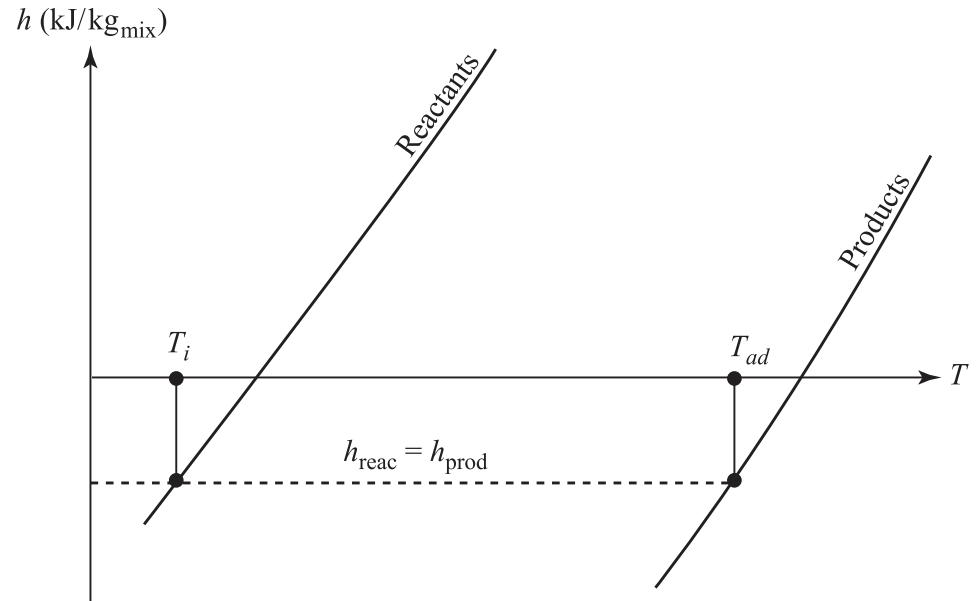
\includegraphics[width=.23\textwidth]{img/ad_T.png}
\end{figure}

\textbf{定容绝热燃烧温度:}反应前后内能相等,
\begin{equation}
    U_{\mathrm{reac}}(T_{\mathrm{init}},P_{\mathrm{init}})=U_{\mathrm{prod}}(T_{a d},P_{f}),
\end{equation}

写成焓的形式:
\begin{equation}
    \begin{aligned}
        H_{\mathrm{reac}}-H_{\mathrm{prod}}-V(P_{\mathrm{init}}-P_{f})&=0.\\
        H_{\mathrm{reac}}-H_{\mathrm{prod}}-R_{u}(N_{\mathrm{reac}}T_{\mathrm{init}}-N_{\mathrm{prod}}T_{a d})&=0.
    \end{aligned}
\end{equation}

\subsection{化学平衡}
\subsubsection{第二定律的讨论}

单个组份的熵计算公式:
\begin{equation}
    \overline{{{s}}}_{i}=\overline{{{s}}}_{i}^{0}(T_{\mathrm{ref}})+\int_{T_{\mathrm{ef}}}^{T_{f}}\overline{{{c}}}_{p,i}\,\frac{\mathrm{d}T}{T}-R_{u}\,\ln\frac{P_{i}}{P^{0}},
\end{equation}

对于封闭系统,反应自发发生的条件为$\mathrm{d}S\ge 0$。平衡条件为:$(\mathrm{d}S)_{U,V,m}=0$。

\subsubsection{吉布斯函数}

单个组份的吉布斯函数的计算:

\begin{equation}
    \overline{{{g}}}_{i,T}=\overline{{{g}}}_{i,T}^{o}+R_{u}T\ln\left(P_{i}/P^{o}\right)
\end{equation}

对于开口系统,我们采用吉布斯函数,它的定义为 $G\equiv H-TS$。这是第二定律表示为$(\mathrm{d}G)_{T,P,m}\le 0$的形式。在平衡时,开口系统的第二定律可以写作$(\mathrm{d}G)_{T,P,m}=0$。

{
    \scriptsize
    考虑广延量,理想气体的吉布斯方程为:
    \[
        G_{\mathrm{mix}}=\sum N_{i}\overline{{{g}}}_{i,T}=\sum N_{i}\bigl[\bar{g}_{i,T}^{0}+R_{u}T\ln\bigl(P_{i}/P^{0}\bigr)\bigr]
    \]
    对上面的式子取微分,得到平衡条件,可以写作:
    \[
        \begin{aligned}
        &\sum{\mathrm{d}{N}}_{i}\left[\bar{g}_{i,T}^{0}+R_{u}T\ln\left(P_{i}/P^{0}\right)\right]+\\
        &\sum{N}_{i}\mathrm{d}\left[\bar{g}_{i,T}^{0}+R_{u}T\ln\left(P_{i}/P^{0}\right)\right]=0.
        \end{aligned}
    \]
    考虑到总压不变,也就是分压变化的和不变,因此式子中的第二项等于零,它可以被简化为:
    \[\sum{\mathrm{d}{N}}_{i}\left[\bar{g}_{i,T}^{o}+R_{u}T\ln\left(P_{i}/P^{0}\right)\right]=0\]
    对于一个一般的系统,我们将化学反应写作
    \[a\mathbf{A}+b\mathbf{B}+\cdots\leftrightarrow e\mathbf{E}+f\mathbf{F}+\cdots\]
    由于物质的摩尔数变化和化学计量数成正比,因此我们可以将平衡表达式展开写作:
    \[
        \begin{aligned}
            &-a\Bigl[\bar{g}_\mathrm{A,T}^{o}+R_{u}T\ln\bigl(P_{\mathrm{A}}/P^{o}\bigr)\Bigr]\\
            &-b\Bigl[\bar{g}_{\mathrm{B,T}}^{o}+R_{u}T\ln\bigl(P_{\mathrm{B}}/P^{o}\bigr)\Bigr]-\cdots\\
            &+e\Bigl[\overline{{{g}}}_{\scriptscriptstyle\mathrm{E,}T}^{o}+R_{u}T\ln\bigl(P_{\scriptscriptstyle\mathrm{E}}/P^{o}\bigr)\Bigr]\\
            &+f\Bigl[\overline{{{g}}}_{\scriptscriptstyle\mathrm{F,}T}^{o}+R_{u}T\ln\bigl(P_{\scriptscriptstyle\mathrm{F}}/P^{o}\bigr)\Bigr]+\cdots=0.
        \end{aligned}
    \]
    合并整理一下不难得到:
    \[
        \begin{aligned}
            &-\Bigl(e\bar{g}_{\mathrm{E},T}^{o}+f\overline{{{g}}}_{\mathrm{F},T}^{o}+\cdot\cdot\cdot-a\overline{{{g}}}_{\mathrm{A},T}^{o}-b\overline{{{g}}}_{\mathrm{B},T}^{o}-\cdots\Bigr)\\
            &=R_{u}T\ln{\frac{\left(P_{\mathrm{E}}/P^{o}\right)^{e}\cdot\left(P_{\mathrm{F}}/P^{o}\right)^{f}\cdot\mathrm{etc.}}{\left(P_{\mathrm{A}}/P^{o}\right)^{a}\cdot\left(P_{\mathrm{B}}/P^{o}\right)^{b}\cdot\mathrm{etc.}}}
        \end{aligned}\]
}
我们定义\textbf{标准状态吉布斯函数差 $\Delta G_T^0$}为:
\begin{equation}
    \Delta G_T^0 = (e\bar{g}_{\mathrm{E},T}^{o}+f\overline{{{g}}}_{\mathrm{F},T}^{o}+\cdot\cdot\cdot-a\overline{{{g}}}_{\mathrm{A},T}^{o}-b\overline{{{g}}}_{\mathrm{B},T}^{o}-\cdots)
\end{equation}
\textbf{平衡常数 \(K_p\)}为:
\begin{equation}
    K_{p}={\frac{\left(P_{\mathrm{E}}/P^{o}\right)^{e}\cdot\left(P_{\mathrm{F}}/P^{o}\right)^{f}\cdot\mathrm{etc.}}{\left(P_{\mathrm{A}}/P^{o}\right)^{a}\cdot\left(P_{\mathrm{B}}/P^{o}\right)^{b}\cdot\mathrm{etc.}}}.
\end{equation}
这时,定压,定温条件下的化学平衡表达式就可以被写作:
\begin{equation}
    \Delta G_T^0 = -R_u T\ln K_p
\end{equation}
\begin{itemize}
    \item 如果\(\Delta G_T^0\)大于零,那么\(K_p\)小于1,反应向左进行(偏向反应物、几乎不反应)。
    \item 如果\(\Delta G_T^0\)小于零,那么\(K_p\)大于1,反应向右进行(偏向产物,趋于完全反应)。
\end{itemize}

{
    \scriptsize
    如果将\(\Delta G_T^0\)写作:
    \[
        \Delta G_T^0 = \Delta H^0 - T\Delta S^0
    \]
    的形式,平衡常数可以被写作:
    \[
        K_p = \mathrm{e}^{-\Delta H^0/R_u T}\cdot \mathrm{e}^{\Delta S^0/R_u}
    \]
    不难发现,
    \begin{itemize}
        \item 当反应的焓变小于零,反应放热,系统能量降低;
        \item 熵变大于零。
    \end{itemize}都会导致反应偏向于产物,\(K_p>1\)。
}

\subsubsection{复杂系统}

\subsection{燃烧的平衡产物}
\subsubsection{全平衡}
考虑实际的燃烧过程,最大燃烧温度一般发生在略微富燃料当量比的状态(\(\Phi\approx 1.05)\)。

\section{传质引论}
\subsection{概述}
\subsection{传质入门}
\subsubsection{传质速率定律}
\begin{itemize}
    \item 菲克扩散定律
    对于一维双组份扩散的情况:
    \begin{equation}\label{equ:fick_law_1d}
        \dot{m}_A'' = Y_A(\dot{m}_A'' + \dot{m}_B'') - \rho \mathcal{D}_\mathrm{AB}\frac{\dd Y_A}{\dd x}
    \end{equation}{\tiny 这里要特别注意,虽然\(\dot{m}_A'' + \dot{m}_B''=\dot{m}''\),但并不意味者\(Y_A \dot{m}''\)就等于\(\dot{m}_A''\)。因为当中还涉及到了扩散作用。}

    \textbf{质量通量}的定义为垂直于流动方向的单位面积质量流量:
    \begin{equation}
        \dot{m}_A'' = \dot{m}_A/A.
    \end{equation}

    可以写成更一般的形式:

    \begin{equation}
        \dot{m}_{\mathrm{A}}^{\prime\prime}=Y_{\mathrm{A}}\,(\dot{m}_{\mathrm{A}}^{\prime\prime}+\dot{m}_{\mathrm{B}}^{\prime\prime})-\rho D_{\mathrm{AB}}\nabla Y_{\mathrm{A}},
    \end{equation}
    \begin{equation}
        \dot{N}_{\mathrm{A}}^{\prime\prime}=\chi_{\mathrm{A}}(\dot{N}_{\mathrm{A}}^{\prime\prime}+\dot{N}_{\mathrm{B}}^{\prime\prime})-c D_{\mathrm{AB}}{\nabla}\chi_{\mathrm{A}},
    \end{equation}
    
    其中\(c\)是混合物的浓度(kmol/m\(^3\))。

    如果我们同时考虑A和B的扩散,将两个物质的式~\ref{equ:fick_law_1d}相加,可以得到:

    \begin{equation}
        -\rho\mathcal{D}_\mathrm{AB}\frac{\dd Y_A}{\dd x} - \rho\mathcal{D}_\mathrm{BA}\frac{\dd Y_B}{\dd x} = 0
    \end{equation}

    \item 扩散的分子基础
    扩散系数和温度及压强的关系:
    \begin{equation}
        \mathcal{D}_\mathrm{AB} \propto T^{3/2}P^{-1}
    \end{equation}

    而质量通量实质上是和\(\rho \mathcal{D}_\mathrm{AB}\)相关,它仅和温度相关:
    \begin{equation}
        \rho\mathcal{D}_\mathrm{AB}\propto T^{1/2}
    \end{equation}
    \item 与热传导的比较
\end{itemize}

\subsubsection{组分守恒}
考虑化学反应:
\begin{equation}
    \frac{\dd m_{\mathrm{A}, cv}}{\dd t} = [\dot{m}_A'' A]_x - [\dot{m}_A'' A]_{x+\Delta x} + \dot{m}_A''' V
\end{equation}

经过整理可以得到:
\begin{equation}
    \frac{\pp(\rho Y_A)}{\pp t} = -\frac{\pp}{\pp x}\left[Y_A\dot{m}'' - \rho \mathcal{D}_\mathrm{AB}\frac{\pp Y_A}{\pp x}\right] + \dot{m}_A'''
\end{equation}

对于稳态的情况:
\begin{equation}
    \dot{m}_A''' - \frac{\dd}{\dd x}\left[Y_A\dot{m}'' - \rho\mathcal{D}_\mathrm{AB}\frac{\dd Y_A}{\dd x}\right] = 0.
\end{equation}

把括号里面的东西打包的话其实也可以写作:
\begin{equation}
    \dot{m}_A''' - \nabla\cdot \dot{m}_A'' = 0
\end{equation}

\subsection{传质的应用实例}
\subsubsection{斯蒂芬问题}

% \begin{figure}[H]
%     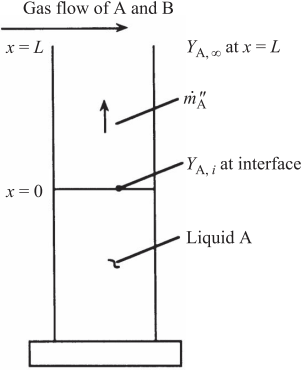
\includegraphics[width=.3\textwidth]{img/stefan.png}
% \end{figure}

我们考虑液体A在玻璃圆通内保持一个固定的高度,假设B在A中不可溶解,由此圆柱中存在着一个B的滞止层。对于这个问题,A的质量通量为:

{\tiny\begin{equation}
    \dot{m}''_A = \frac{\rho \mathcal{D}_\mathrm{AB}}{L}\ln\left(\frac{1-Y_{A,\infty}}{1-Y_{A,i}}\right)
\end{equation}
}
推导过程如下:
{\scriptsize\color{gray}

由于B的量通量为0,基于菲克定律式~\ref{equ:fick_law_1d},我们可以写出
\[
    \dot{m}_A'' = Y_A\dot{m}_A'' - \rho \mathcal{D}_\mathrm{AB}\frac{\dd Y_A}{\dd x}
\]对之整理并分离变量:
\[
    -{\frac{\dot{m}_{\mathrm{A}}^{\prime\prime}}{\rho D_{\mathrm{AB}}}}\mathrm{d}x={\frac{\mathrm{d}Y_{\mathrm{A}}}{1-Y_{\mathrm{A}}}}.
\]
积分解得:
\[
    -{\frac{\bar{m}_{\mathrm{A}}^{\prime\prime}}{\rho D_{\mathrm{AB}}}}\,x=-\ln[1-Y_{\mathrm{A}}]+C,
\]结合已知边界条件,\(Y_A(x=0)=Y_{A,i}, Y_A(x=L)=Y_{A,\infty}\)。}

就可以写出质量分数的计算公式:

\begin{equation}
    Y_A(x) = 1 - (1-Y_{A,i})\exp\left(\frac{\dot{m}_A'' x}{\rho\mathcal{D}_\mathrm{AB}}\right)
\end{equation}

\subsubsection{液-气界面的边界条件}

不难写出\(\chi_{A,i} = P_\mathrm{sat}/P\),由此可以确定质量分数应该为:
\begin{equation}
    Y_{A,i} = \frac{P_\mathrm{sat}(T_\mathrm{liq, i})}{P}\frac{\mathrm{MW}}{\mathrm{MW}_\mathrm{mix, i}}
\end{equation}

认为液-气界面上维持温度的连续性,那么:
\[
    T_\mathrm{liq,i}(x=0^-) = T_\mathrm{vap, i}(x=0^+) = T(0)
\]


\subsubsection{液滴蒸发}

\textbf{假设}:
{\scriptsize
    \begin{enumerate}
        \item 蒸发过程是准稳态的。
        \item 液滴的温度均一,进而假设温度为低于液体的沸点的某一定值。
        \item 液滴表面蒸气的质量分数由液滴温度下的液体-蒸气平衡确定。
        \item 假设所有的热物理参数——特别是\(\rho\mathcal{D}\)——是常数。
    \end{enumerate}
}

\textbf{蒸发速率}:

从某种意义上说,这里的液滴蒸发问题其实就是一个加强版的球状的斯蒂芬流。定义\textbf{传质数}\(B_Y\)为:
\begin{equation}
    B_Y = \frac{Y_{A,s}-Y_{A,\infty}}{1 - Y_{A,s}}
\end{equation}
蒸发速率可以被写作:
\begin{equation}\label{equ:evo_rate}
    \dot{m}_A''' = {4\pi r_s \rho \mathcal{D}_\mathrm{AB}}\ln({1+B_Y})
\end{equation}

具体的推倒过程如下所示:

{
    \scriptsize\color{gray}
    首先,液滴的蒸发速率可以被写作
    \[
        \dot{m}(r) = 4\pi r^2 \dot{m}''
    \]
    将之带入到菲克定律~\ref{equ:fick_law_1d}的表达式中,并且认为另一组份滞止,可以得到:
    \[
        \dot{m}_A'' = Y_A\dot{m}_A'' - \rho\mathcal{D}_\mathrm{AB}\frac{\dd Y_A}{\dd r}
    \]
    代入蒸发速率的表达式,并且整理,可以得到:
    \[
        \dot{m}=-4\pi r^2 \frac{\rho \mathcal{D}_\mathrm{AB}}{1-Y_A}\frac{\dd Y_A}{\dd r}
    \]
    首先代入液滴表面的边界条件\(Y_A(r=r_s)=Y_{A,s}\),可以得到:
    \[
        Y_{\mathrm{A}}(r)=1-{\frac{(1-Y_{\mathrm{A,s}})\exp[-\dot{m}/(4\pi\rho \mathcal{D}_{\mathrm{AB}}r)]}{\exp[-\dot{m}/(4\pi\rho \mathcal{D}_{\mathrm{AB}}r_{s})]}}.
    \]
    再代入\(r\to\infty\)时,\(Y_A=Y_{A,\infty}\),可以解得蒸发速率\(\dot{m}\)的最终结果。
}

\textbf{液滴质量守恒}:

显然,液滴质量和蒸发速率之间的关系是:

\begin{equation}
    \frac{\dd m_d}{\dd t}=-\dot{m}
\end{equation}
液滴的质量可以写作:
\begin{equation}
    m_d = \rho_l V = \rho_l \pi D^3/6
\end{equation}
将这两个式子代入到液滴蒸发速率的公式中(式~\ref{equ:evo_rate}),化简唯粉整理,可以得到:
\begin{equation}
    \frac{\mathrm{d}D}{\mathrm{d}t}=-\frac{4\rho \mathcal{D}_\mathrm{AB}}{\rho_{i}D}\mathrm{ln}(1+B_{Y}).
\end{equation}
或者是:
\begin{equation}
    {\frac{\mathrm{d}D^{2}}{\mathrm{d}t}}=-{\frac{8\rho \mathcal{D}_{\mathrm{AB}}}{\rho_{l}}}\ln(1+B_{Y}).
\end{equation}

我们将等式的右边定义为\textbf{蒸发常数}:
\begin{equation}
    K = {\frac{8\rho \mathcal{D}_{\mathrm{AB}}}{\rho_{l}}}\ln(1+B_{Y})
\end{equation}

由此可以得到\(D\)随时间\(t\)的关系式:
\begin{equation}
    D^2(t)=D_0^2 - Kt
\end{equation}
这就是\textbf{\(D^2\)定律}。

\begin{figure}[H]
    \centering
    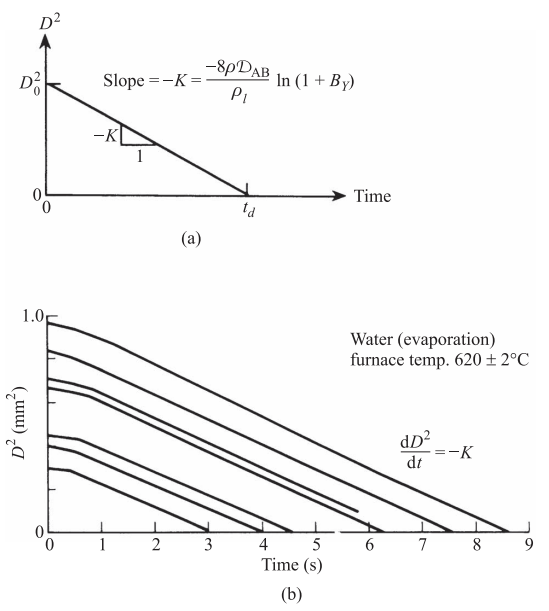
\includegraphics[width=.3\textwidth]{img/d2.png}
\end{figure}

\section{化学动力学}
\subsection{概述}
\subsection{总包反应与基元反应}
燃料和氧化剂的\textbf{总包反应机理}可以被写作:
\begin{equation}
    \mathrm{F} + a\mathrm{Ox}\leftarrow b\mathrm{Pr}
\end{equation}

反应速率可以被表达为:

\begin{equation}
    {\frac{\mathrm{d}[X_{F}]}{\mathrm{d}t}}=-k_{G}(T)[X_{F}]^{n}[X_{O x}]^{m},
\end{equation}其中\(k_G\)为\textbf{总包反应速率常数},\(n\), \(m\)为\textbf{反应级数}。这个式子只在特定的温度和压力范围适用,并且与用于确定反应速率参数的实验装置有关。为了描述一个总体反应所需要的一组基元反应称为\textbf{反应机理}.

\textbf{基团}或\textbf{自由基}是指具有反应性的分子或原子,拥有不成对的电子。

\subsection{基元反应速率}
\subsubsection{双分子反应和碰撞理论}
大部分的基元反应是\textbf{双分子反应}:

\begin{equation}
    \mathrm{A}+\mathrm{B}\rightarrow \mathrm{C} + \mathrm{D}
\end{equation}

反应速率可以写作:
\begin{equation}
    {\frac{\mathrm{d}[{A}]}{\mathrm{d}t}}=-k_{\mathrm{bimolec}}[{A}][{B}].
\end{equation}
如果研究问题的温度范围不是很大,双分子反应速率常数可以用经验的阿累尼乌斯形式(Arrheniusform)来表示,即:
\begin{equation}
    k(T) = A\exp(-E_A/R_u T)
\end{equation}这里的\(A\)是\textbf{指前因子}或\textbf{频率因子}。严格来说它与\(T^{1/2}\)相关。

也有写作:
\begin{equation}
    k(T)=A T^{b}\exp(-E_{A}/R_{u}T),
\end{equation}

\subsubsection{其他基元反应}

\textbf{单分子反应:}
\begin{equation}
    \mathrm{A\rightarrow B}
\end{equation}
或者:
\begin{equation}
    \mathrm{A}\rightarrow \mathrm{B} + \mathrm{C}
\end{equation}

在高压的情况下,这个反应是一阶的,反应速率为:
\begin{equation}
    \frac{\dd \mathrm{A}}{\dd t}=-k_{\mathrm{uni}}[\mathrm{A}]
\end{equation}
在低压时,它还与任意分子的浓度有关,
\begin{equation}
    \frac{\dd[\mathrm{A}]}{\dd t}=-k[\mathrm{A}][\mathrm{M}]
\end{equation}这里的M是任意分子。

\textbf{三分子反应}
\begin{equation}
    \mathrm{A + B + M \rightarrow C + M}
\end{equation}

这里的M同样是任意分子。

\textbf{第三体的作用}:在自由基-自由基反应中,第三体的作用是携带走在形成稳定的组分时释放出来的能量。在碰撞的过程中,新形成的分子的内能传递给第三体 M,成为 M 的动能。没有这一能量的传递,新形成的分子将重新离解为组成它的原子。

\subsection{多步反应机理的反应速率}
\subsubsection{净生成率}
\subsubsection{净生成率的简洁表达式}
对于反应机理,表达式可以写为
\begin{equation}
    \sum_{j=1}^{N}\nu_{j}^{\prime}\,X_{j}\Leftrightarrow\sum_{j=1}^{N}\nu_{j i}^{\prime\prime}\,X_{j}\quad{\mathrm{for}}\quad i=1,2,\dots,L\,,
\end{equation}
净生成率被写作:
\begin{equation}
    \dot{\omega_j}=\sum_{i=1}^L\nu_{ji} q_i\quad{\mathrm{for}}\quad j=1,2,\dots,N\,,
\end{equation}
\begin{equation}
    \nu_{ji} = (\nu_{ji}'' - \nu_{ji}')
\end{equation}
\begin{equation}
    q_i = k_{fi}\Pi_{j=1}^N[X_j]^{\nu_{ji}'} - k_{ri}\Pi_{j=1}^N[X_j]^{\nu_{ji}''}
\end{equation}

\subsubsection{反应速率常数与平衡常数之间的关系}
速率常数不好测,基于热力学测量与计算的平衡常数好测。

\begin{equation}
    \frac{k_f(T)}{k_r(T)} = K_c(T)
\end{equation}

这里的\(K_c\)是基于浓度的平衡常数:
\[K_p = K_c (R_u T/ P^0)^{c+d+\cdots-a-b-\cdots}=K_c (R_u T/ P^0)^{\sum \nu''-\sum \nu'}\]

实际操作中,测定好测的正反应速率常数,然后推算出逆反应的速率常数。

\subsubsection{稳态近似}
在燃烧过程所涉及的许多化学反应系统中,会形成许多高反应性的中间产物,即自由基。针对这类中间产物或自由基,采用稳态近似,就可以大大减少对这些系统的分析工作。从物理上讲,这些自由基的浓度在一个迅速的初始增长后,其消耗与形成的速率就很快趋近,即生成和消耗速率是相等的。

\subsubsection{单分子反应机理}

考虑第三体的作用,产物的生成速率应当等于激活的A分子浓度成一阶反应的速率常数:

\begin{equation}
    \frac{\dd[\mathrm{products}]}{\dd t}=k_\mathrm{uni}[\mathrm{A^*}]
\end{equation}

利用稳态近似,认为激活的A分子浓度不变,可以将A\(^*\)的净生成率表达成为:

\begin{equation}
    {\frac{\mathrm{d}[\mathrm{A}^{*}]}{\mathrm{d}t}}=k_{e}[\mathrm{A}][\mathrm{M}]-k_\mathrm{d e}[\mathrm{A}^{*}][\mathrm{M}]-k_{\mathrm{uni}}[\mathrm{A}^{*}].
\end{equation}

经过层层推导可以得到如下的结论:

\begin{equation}\label{equ:unimol_react}
    -\frac{\dd[\mathrm{A}]}{\dd t}=\frac{\dd[\mathrm{products}]}{\dd t} = k_\mathrm{app}[\mathrm{A}]
\end{equation}其中\(k_\mathrm{app}\)被定义为单分子反应的\textbf{表观速率常数},计算公式为:

\begin{equation}
    k_\mathrm{app}=\frac{k_e[\mathrm{M}]}{(k_\mathrm{de}/k_\mathrm{uni})[\mathrm{M}]+1}
\end{equation}

\subsubsection{链式反应和链式分支反应}

对于总包反应

\begin{equation}
    \mathrm{A_2+B_2}\rightarrow 2\mathrm{AB}
\end{equation}

\textbf{链的激发反应}为:
\begin{equation}
    \mathrm{A_2+M}\overset{k_1}{\longrightarrow} \mathrm{A+A+M}
\end{equation}
\textbf{链的传播反应}为:
\begin{eqnarray}
    \mathrm{A+B_2\overset{k_2}{\longrightarrow}AB + B}\\
    \mathrm{B+A_2\overset{k_3}{\longrightarrow}AB + A}
\end{eqnarray}
\textbf{链的终止反应}为:
\begin{equation}
    \mathrm{A+B+M\overset{k_4}{\longrightarrow}AB+M}
\end{equation}

分析过程太复杂,可以看书100页。几个结论:
\begin{equation}
    [\mathrm{A}]\approx{\frac{[\mathrm{A}_{2}]}{[\mathrm{B}_{2}]^{1/2}}}\left({\frac{k_{1}k_{3}}{k_{2}k_{4}}}\right)^{1/2}
\end{equation}

\begin{equation}
    \frac{\mathrm{d}[{\mathrm{B}}_{2}]}{\mathrm{d}t}\approx-[{\mathrm{A}}_{2}][{\mathrm{B}}_{2}]^{1/2}\left(\frac{k_{1}k_{2}k_{3}}{k_{4}}\right)^{1/2}.
\end{equation}
\begin{enumerate}
    \item 链的激发反应速率越大,链的中断反应速率常数越小,自由基的浓度也越大。
    \item 增大链的传递反应速率常数,会增大\([\mathrm{B_2}]\)的消耗速率。
    \item 链的传递反应速率常数对自由基的浓度影响不大。因为由于其速率常数具有相同的量级且以一个比值的方式出现。
\end{enumerate}

压力足够高时,由于假设的\(4k_2 k_3[B_2]/(k_1 k_4[M]^2)\gg 1\)不再成立,上面的结论也不再可靠。

\textbf{链式分支反应}是指:\textit{消耗一个}自由基而\textit{形成两个}自由基组分的反应。链式分支反应对具有自传播特性的火焰起主导作用,这也是燃烧化学中最基本的特征。

\textbf{化学时间尺度}

\begin{enumerate}
    \item 单分子反应
    我们对单分子反应速率的表达式\ref{equ:unimol_react}进行积分,得到:
    \begin{equation}
        [\mathrm{A}](t)=[\mathrm{A}]_{0}\exp(-k_{\mathrm{app}}t)
    \end{equation}其中[A]\(_0\)为组份A的初始浓度. 如果用RC电路定义特征时间的方法,我们可以得到\textbf{化学时间尺度}的表达式:
    \begin{equation}
        \tau_\mathrm{chem} = 1/k_\mathrm{app}
    \end{equation}

    \item 双分子反应
    对于如下的反应
    \[
        \mathrm{A+B\rightarrow C+D}
    \]
    它的速率表达式为:
    \begin{equation}
        \frac{\dd [\mathrm{A}]}{\dd t}=-k_\mathrm{bimolec}\mathrm{[A][B]}
    \end{equation}
    A和B的浓度变化可以通过化学当量关系来联系, 经过推导之后最后得到结论:
    \begin{equation}
        \tau_{\mathrm{chem}}={\frac{\mathrm{ln}[e+(1-e)\mathrm{([A]_{0}/[B]_{0})}]}{([\mathrm{B}]_{0}-\mathrm{[A]}_{0})k_{\mathrm{bimodec}}}},
    \end{equation}其中\(e=2.718\).

    如果其中反应物浓度要比另一种大得多,比如B很大,那么上面的式子可以简化为:
    \begin{equation}
        \tau_\mathrm{chem}=\frac{1}{[\mathrm{B}]_0 k_\mathrm{bimolec}}
    \end{equation}

    \item 三分子反应
    \[\mathrm{A+B+M\rightarrow C + M}\]
    如果我们认为第三体浓度[M]是一个常数,我们可以得到和双分子反应类似的结论:
    \begin{equation}
        {\frac{\mathrm{d}[\mathrm{A}]}{\mathrm{d}t}}=(-k_{\mathrm{ter}}[\mathrm{M}])[\mathrm{A}][\mathrm{B}].
    \end{equation}

    \begin{equation}
        \tau_{\mathrm{chem}}={\frac{\mathrm{ln}[e+(1-e)([\mathrm{A}]_{0}/[\mathrm{B}]_{0})]}{([\mathrm{B}]_{0}-[\mathrm{A}]_{0})k_{\mathrm{te}}[\mathrm{M}]}},
    \end{equation}


    类似地, 如果B的浓度远远大于A, 那么:
    \begin{equation}
        \tau_{\mathrm{chem}}=\frac{1}{[{\rm B}]_{0}[{\rm M}]k_{\mathrm{ter}}}.
    \end{equation}
\end{enumerate}

\subsubsection{部分平衡}
将\textit{快速反应}视作\textit{平衡态}处理可以简化化学动力学机理,从而无须写出所涉及自由基的速率方程。这种处理方法叫作部分\textbf{平衡近似}。

\section{一些重要的化学机理}

\subsection{概述}
\subsection{\(\mathrm{H_2-O_2}\)系统}

\begin{multicols}{2}
{\fontsize{4}{1}\selectfont
初始激发反应(第一个为高温, 第二个为其他温度):
\begin{eqnarray}
    \mathrm{H_2+M}&\to&\mathrm{H+H+M}\\
    \mathrm{H_2+O_2}&\to&\mathrm{HO_2+H}\label{equ:activate}
\end{eqnarray}
包含有自由基 0,H 和 OH 的链式反应是:
\begin{eqnarray}
    \mathrm{H+O_2}&\to& \mathrm{O+OH}\label{equ:chain1}\\
    \mathrm{O + H_2}&\to& \mathrm{H + OH}\\
    \mathrm{H_2+OH}&\to& \mathrm{H_2O+H}\\
    \mathrm{O+H_2O}&\to& \mathrm{OH+OH}\label{equ:chain4}
\end{eqnarray}
包含自由基 O,H 和 OH 自由基的链的中断反应是三分子化合反应
\begin{eqnarray}
    \mathrm{H+H+M}&\to&\mathrm{H_2+M}\\
    \mathrm{O+O+M}&\to& \mathrm{O_2+M}\\
    \mathrm{H+O+M}&\to& \mathrm{OH + M}\\
    \mathrm{H + OH + M} &\to& \mathrm{H_2O + M}
\end{eqnarray}

过氧羟基和双氧水的反应也很重要, 当这个反应变得活跃是:
\begin{equation}\label{equ:HO2}
    \mathrm{H+O_2+M}\to \mathrm{HO_2 +M}
\end{equation}

下列反应和第二个反应的逆反应开始起作用:
\begin{eqnarray}
    \mathrm{HO_2+H} &\to& \mathrm{OH+OH} \\
    \mathrm{HO_2+H} &\to& \mathrm{H_2O+O} \\
    \mathrm{HO_2+O} &\to& \mathrm{O_2+OH} \\
    \mathrm{HO_2+HO_2} &\to& \mathrm{H_2O_2+O_2} \\
    \mathrm{HO_2+H_2} &\to& \mathrm{H_2O_2+H} \label{equ:H2O2}\\
    \mathrm{H_2O_2+OH} &\to& \mathrm{H_2O+HO_2} \\
    \mathrm{H_2O_2+H} &\to& \mathrm{H_2O+OH} \\
    \mathrm{H_2O_2+H} &\to& \mathrm{HO_2+H_2} \\
    \mathrm{H_2O_2+M} &\to& \mathrm{OH+OH+M}
\end{eqnarray}
}
\end{multicols}
关于书本图5.1爆照极限的分析(500$^\circ$C 这一条线来讨论爆炸行为):
\begin{enumerate}
    \item 小于1.5 mmHg, 无爆炸,这是因为~\ref{equ:activate}激发的步骤和后面的链式反应~\ref{equ:chain1}-\ref{equ:chain4}所产生的自由基被避免反应所消耗而中断.
    \item 高于1.5 mmHg爆炸就会发生是因为\ref{equ:chain1}-\ref{equ:chain4}所产生的自由基超过了壁面的消耗速度(压力增加导致自由基的浓度呈线性增加,相应的反应速率呈几何增加。).
    \item 高于50 mmHg时, 混合物又停止了爆炸的特性, 这是由于链式分支反应~\ref{equ:chain1}和低温下显著的链中断反应~\ref{equ:HO2}之间产生了竞争. 过氧羟基相对不活跃, \ref{equ:HO2}可以被看作是链中断反应, 产生的自由基扩散到了壁面被消耗.
    \item 高于3000 mmHg时, \ref{equ:H2O2}加入到了链式分支反应中,引起了双氧水的链式反应过程.
\end{enumerate}

\subsection{一氧化碳的氧化}

不含水时,一氧化碳的氧化非常缓慢, 少量水的影响非常大, 因为羟基很重要.

\begin{eqnarray}
    \mathrm{CO+O_2} &\to& \mathrm{CO_2+O} \\
    \mathrm{O + H_2O} &\to& \mathrm{OH + OH} \\
    \mathrm{CO + OH} &\to& \mathrm{CO_2 + H} \label{equ:CO_burn}\\
    \mathrm{H + O_2} &\to& \mathrm{OH + O}
\end{eqnarray}

第一个反应激发链式反应, CO的实际氧化通过第三个反应完成.

如果催化剂为氢气, 那么还会包括氢气和氧原子, 氢气和羟基的反应. 实质上, 在有氢的情况下,为了描述CO的氧化, 需要包含上面提到的所有氢氧反应. 此外, 在过氧羟基存在的基础上, 还需要包括它氧化CO生成水和二氧化碳的反应.

\subsection{碳氢化合物的氧化}
碳氢化合物的燃烧可以简单地分为两步:第一步包括燃料断裂生成一氧化碳;第二步是一氧化碳最终氧化成为二氧化碳。

\subsubsection{链烷烃概况}

链烷烃, aka. 石蜡类物质, 化学分子式\(\mathrm{C_n H_{2n+2}}\). 这里先讨论\(n>2\)的情况.
\begin{enumerate}
    \item  燃料分子受到O和H原子的撞击而分解,先分解成烯烃和氢。在有氧存在的情况
下,氢就氧化成水。
    \item 不饱和烯烃进一步氧化成为CO和\(\mathrm{H_2}\), 所有的\(\mathrm{H_2}\)都转化为水.
    \item CO通过~\ref{equ:CO_burn}燃尽, 热量主要在这一步释放.
\end{enumerate}

具体展开如下:
\begin{enumerate}
    \item 薄弱的C-C键先于C-H键断裂, 产生碳氢自由基.
    \item \textbf{脱氢}: 碳氢自由基进一步分解, 产生烯烃和氢原子.
    \item 上一步中的氢原子进一步产生新的自由基(羟基和氧原子).
    \item 自由基的累计开始了新的燃料分子被撞击的过程.
    \item 生成的碳氢自由基进一步脱氢(基于\(\beta\)剪刀原则展开).
    \item 烯烃由O原子撞击产生氧化, 生成甲酸基(HCO)和甲醛(H\(_2\)CO).
    \item 甲基, 甲醛, 亚甲基氧化,
    \item 按含湿的 CO 机理进行的一氧化碳的氧化.
\end{enumerate}

\textbf{\(\beta\)剪刀原则:} 断裂C-C或C-H键将是离开自由基位置的一个键(离开不成对电子的一个位置). 这是因为在自由基位置处的不成对电子加强了相邻的键, 导致了从这一位置向外移动了一个位置.

\subsubsection{总包和准总包机理}

一步总包:
\begin{equation}
    \mathrm{C}_x \mathrm{H}_y + (x+y/4)\mathrm{O_2} \to x\mathrm{CO_2} + y/2\mathrm{H_2O}
\end{equation}

四步反应模拟丙烷的氧化:
\begin{enumerate}
    \item \(\mathrm{C}_n \mathrm{H}_{2n+2} \to (n/2) \mathrm{C}_2 \mathrm{H}_4 + \mathrm{H}_2\)
    \item \(\mathrm{C}_2\mathrm{H}_4 + \mathrm{O}_2 \to 2\mathrm{CO} + 2 \mathrm{H}_2\)
    \item \(\mathrm{CO+\frac{1}{2}O_2\to CO_2}\)
    \item \(\mathrm{H_2 + \frac{1}{2}O_2\to H_2O}\)
\end{enumerate}

\subsubsection{实际燃料及其替代物}

\subsection{甲烷燃烧}
\subsubsection{复杂机理}
\subsubsection{高温反应途径分析}
\begin{enumerate}
    \item 主线从OH, O和H撞击CH\(_4\)产生甲基自由基开始;
    \item 甲基自由基和氧原子产生甲醛;
    \item 甲醛由OH, H和O撞击形成甲酸基;
    \item 甲酸基通过三个反应形成CO;
    \item CO变成CO\(_2\).
\end{enumerate}

除了这一途径, 还有一些其他途径:
\begin{enumerate}
    \item 甲基形成两种可能电子结构的亚甲基
    \item 甲基形成甲醇, 然后变成甲醛.
\end{enumerate}
\subsubsection{低温反应途径分析}
几个有趣现象:
\begin{enumerate}
    \item 存在较强的甲基重新变成甲烷的现象;
    \item 通过甲醇, 出现了从甲基到甲醛的新途径;
    \item 甲基变成了乙烷, 乙烷变成乙烯和乙炔然后变成一氧化碳和亚甲基(出现比初始弹琴化合物高的碳氢化合物是低温氧化过程的一个共同特点).
\end{enumerate}

\subsection{氮氧化物的形成}

\begin{enumerate}
    \item \textbf{热力型机理}在高温燃烧中起支配作用,当量比可以在很宽的范围内变化。
    \item \textbf{费尼莫机理}在富燃料燃烧中特别重要。
    \item \textbf{N\(_2\)O-中间体机理}在很贫的燃料和低温燃烧过程中对 NO 的产生有很重要的作用。
    \item \textbf{NNH机理}相对上面提到的机理是新提出的。
\end{enumerate}

\textbf{热力型机理, Zeldovich}:
\begin{eqnarray}
    \mathrm{O+N_2} &\leftrightarrow& \mathrm{NO + N}\\
    \mathrm{N+O_2} &\leftrightarrow& \mathrm{NO + O}\\
    \mathrm{N+OH} &\leftrightarrow& \mathrm{NO + H}
\end{eqnarray}
按理说这个反应会通过氧气, 羟基和氧原子与燃烧发生耦合. 但是由于一般只有在燃烧完全后, NO的形成才会明显, 所以他们一般不耦合. 在此情况下, 如果认为
\begin{enumerate}
    \item 反应尺度够长\(\to\)氮气, 氧气, 氧原子和羟基浓度处于平衡值;
    \item NO浓度远小于平衡值\(\to\)逆反应忽略
\end{enumerate}

那么NO的生成就只和氧原子和氮气相关.

当然在火焰区, 时间尺度小, 平衡假设不成立. 此时O处于超平衡浓度, 大大加快了NO的形成速率(有时归结为快速型NO机理, 考虑历史, 快速限定为费尼莫尔机理).
由于活化能大, 所以高温下此机理才重要. 又由于时间尺度小于燃料氧化的时间尺度, 因此NO往往在火焰后的气体中产生.

\textbf{N\(_2\)O-中间体机理}
在贫燃料(\(\phi<0.8\))和低温的条件下, N\(_2\)O-中间体机理很重要 (燃气轮机制造商):

\begin{eqnarray}
    \mathrm{O + N_2 + M} &\leftrightarrow& \mathrm{N_2O + M}\\
    \mathrm{H + N_2O} &\leftrightarrow& \mathrm{NO + NH}\\
    \mathrm{O + N_2O} &\leftrightarrow& \mathrm{NO + NO}
\end{eqnarray}


\textbf{费尼莫尔机理/快速型NO}
得名原因: 费尼莫尔最早发现 NO 在层流预混火焰的火焰区域中快速地产生,且是在热力型 NO 形成之前就已形成。
\begin{eqnarray}
    \mathrm{CH + H_2} &\leftrightarrow& \mathrm{HCN + N}\\
    \mathrm{C + N_2} &\leftrightarrow& \mathrm{CN + N}
\end{eqnarray}

在当量比小于1.2时, HCN由下面的方法产生NO:

\begin{eqnarray}
    \mathrm{HCN + O} &\leftrightarrow& \mathrm{NCO + H} \\
    \mathrm{NCO + H} &\leftrightarrow& \mathrm{HN + CO} \\
    \mathrm{NH + H} &\leftrightarrow& \mathrm{N + H_2} \\
    \mathrm{N + OH} &\leftrightarrow& \mathrm{NO + H}
\end{eqnarray}

当量比大于1.2时, 会比较复杂.

如果上面的反应不快速的时候, NO会形成HCN, 然后反应就倒过来了, 氧化变成了还原.

\textbf{NNH机理}: 

对氢的燃烧, 大碳氢比燃料的燃烧很重要:

\begin{eqnarray}
    \mathrm{N_2 + H} &\leftrightarrow& \mathrm{NNH}\\
    \mathrm{NNH + O} &\leftrightarrow& \mathrm{NO + NH}
\end{eqnarray}

\textbf{燃料氮}:

燃料中含有的氮,这些氮形成的NO是燃料氮,也是一个重要的途径。煤里面的氮比较多,可能会生成HCN和NH\(_3\).后面的机理和快速型NO机理差不多.

一氧化氮进入大气以后的事儿,和在进入以前就形成\(\mathrm{NO_2}\)可以看看书146.


\section{反应系统化学与热力学分析的耦合}
\subsection{概述}
\subsection{定压-定质量反应器}
\subsubsection{守恒定律的应用}

考虑焓的变化:
\begin{equation}
    \frac{\dot{Q}}{m} = \frac{\dd h}{\dd t}
\end{equation}

\[
    \begin{aligned}
        h&={\frac{H}{m}}=\sum_{i=1}^{N}N_{i}{\overline{{h_{i}}}}{}\\
        {\frac{\mathrm{d}h}{\mathrm{d}t}}&={\frac{1}{m}}\left[\sum_{i}\left({\overline{{h}}}_{i}\,{\frac{\mathrm{d}N_{i}}{\mathrm{d}t}}\right)+\sum_{i}\left(N_{i}\,{\frac{\mathrm{d}{\overline{{h}}}_{i}}{\mathrm{d}t}}\right)\right].
    \end{aligned}
\]
对于理想气体,我们可以写出:
\[
    {\frac{\mathrm{d}{\tilde{h}}_{i}}{\mathrm{d}t}}={\frac{\partial{\tilde{h}}_{i}}{\partial T}}{\frac{\mathrm{d}T}{\mathrm{d}t}}={\overline{{c}}}_{p,i}\,{\frac{\mathrm{d}T}{\mathrm{d}t}},
\]
对于物质的量的变化:
\[
    \begin{aligned}
        N_i &= V[X_i]\\
        \frac{\dd N_i}{\dd t} &\equiv V\dot{\omega}_i
    \end{aligned}\]
由此,把上面这些式子互相放在一起互相代一下,我们可以得到,关于温度的方程:
\begin{equation}\color{red}\label{equ:reac_p_T}
    {\frac{\mathrm{d}T}{\mathrm{d}t}}={\frac{({\dot{Q}}/V)-\sum_{i}({\bar{h}}_{i}{\dot{\omega}}_{i})}{\sum_{i}([X_{i}]{\overline{{c}}}_{p,i})}},
\end{equation}其中的焓,可以用下面的方程来写:
\begin{equation}
    \overline{{{h}}}_{i}=\overline{{{h}}}_{f,i}^{o}+\sum_{T_\mathrm{ref}}^{T}\overline{{{c}}}_{p,i}\,\mathrm{d}T.
\end{equation}

对于体积的关系,我们需要运用质量守恒,首先,体积和摩尔浓度之间的关系是:
\begin{equation}
    V={\frac{m}{\sum_{i}([X_{i}]M W_{i})}}.
\end{equation}
摩尔分数的变化可以写作:
\begin{equation}
    {\frac{\mathrm{d}[X_{i}]}{\mathrm{d}t}}={\dot{\omega}}_{i}-[X_{i}]{\frac{1}{V}}{\frac{\mathrm{d}V}{\mathrm{d}t}},
\end{equation}
综合运用理想气体方程,消去\(\dd V/\dd t\)项,我们可以得到:

\begin{equation}\color{red}\label{equ:reac_p_X}
    {\frac{\mathrm{d}[X_{i}]}{\mathrm{d}t}}={\dot{\omega}}_{i}-[X_{i}]{\Biggl[}{\frac{\sum{\dot{\omega}}_{i}}{\sum_j [X_j]}}+{\frac{1}{T}}{\frac{\mathrm{d}T}{\mathrm{d}t}}{\Biggr]}.
\end{equation}

\subsubsection{反应器模型小结}

除了公式~\ref{equ:reac_p_T}, \ref{equ:reac_p_X}以外,我们再补上两个初始条件,这个问题就完全闭合了。

\textbf{柴油机 vs. 汽油机}: 按理说,定压定质量的反应容器温度应该更低,因此柴油机的效率看起来会比汽油机要更低一些,但是不能忘记的是,考虑到爆震/敲缸的问题,柴油机的压缩比能做到比汽油机高很多,所以综合考虑下来柴油机的效率会更加高一些。

\subsection{定容-定质量反应器}
\subsubsection{守恒定律的应用}
过程和上次类似,不过是考虑内能的变化:
\[
    \frac{\mathrm{d}T}{\mathrm{d}t}=\frac{({\dot{Q}}/V)-\sum_i({\tilde{u}}_{i}{\dot{\omega}}_{i})}{\sum_{i}([X_{i}]{\overline{{{c}}}}_{\upsilon,i})}.
\]
对于理想气体,我们给他写成有关焓的形式:
\begin{equation}\color{red}\label{equ:reac_v_T}
    {\frac{\mathrm{d}T}{\mathrm{d}t}}={\frac{({\dot{Q}}/V)+R_{u}T\sum{\dot{\omega}}_{i}-\sum_{i}({\dot{h}}_{i}{\dot{\omega}}_{i})}{\sum_{i}[\left[X_{i}|({\overline{{c}}}_{p,i}-R_{u})\right]}}.
\end{equation}

关于摩尔浓度的变化,定容的反应器是不必多说的。压力的变化是一个我们很关心的问题,同样根据理想气体状态方程,压力的变化可以被写作:
\begin{equation}\color{red}\label{equ:reac_v_P}
    {\frac{\mathrm{d}P}{\mathrm{d}t}}=R_{u}T\sum_{i}{\dot{\omega}}_{i}+R_{u}\sum_{i}[X_{i}]{\frac{\mathrm{d}T}{\mathrm{d}t}},
\end{equation}

\subsubsection{反应器模型小结}
除了上面的~\ref{equ:reac_v_T}以外,摩尔浓度的变化可以被写作:

\begin{equation}\color{red}
    {\frac{\mathrm{d}[X_{i}]}{\mathrm{d}t}}={\dot{\omega}}_{i}=f([X_{i}],T)\qquad i=1,\;2,\ldots,N
\end{equation}

我们再补两个初始条件,就完事儿了。

\textbf{敲缸}:在电火花点火发动机中,如果在火焰到达之前,未燃燃料-空气混合物就发生均相反应,会引起敲缸,也就是自动点火。

\subsection{全混反应器}
\subsubsection{守恒定律的应用}

如果我们忽略任何的扩散通量,对于某一特定物质流入流出的质量流的变化应当等于反应器内化学反应生成的该物质,亦即:
\begin{equation}\color{red}\label{equ:reac_stir_omega}
    \dot{\omega}_i MW_i V + \dot{m}(Y_{i, \mathrm{in}} - Y_{i, \mathrm{out}}) = 0\quad{\text{for }i=1,2,\ldots,N~\text{species}}
\end{equation}

对于化学反应部分,由于反应器内部组份处处相等,因此出口的部分应当和内部相同,亦即:
\begin{equation}
    \dot{\omega}_i = f([X_i]_{cv}, T) = f([X_i]_\mathrm{out}, T)
\end{equation}

其中质量分数与物质的量的浓度的关系为:
\begin{equation}
    Y_i = \frac{[X_i] MW_i}{\sum_{j=1}^N [X_j]MW_j}
\end{equation}

目前,对于每一个物质,我们都可以写出一个~\ref{equ:reac_stir_omega},由此我们就有N个方程,如果我们认为入口流量和反应器体积已知,那么我们还缺一个额外的方程去确定反应器的能量状态。

\begin{equation}\color{red}
    \dot{Q}=\dot{m}\left(\sum_{i=1}^{N}Y_{i,\mathrm{out}}h_{i}(T)-\sum_{i=1}^{N}Y_{i,\mathrm{in}}h_{i}(T_{\mathrm{in}})\right),
\end{equation}其中,
\begin{equation}
    h_{i}(T)=h_{f,i}^{o}+\int_{T_{i}(f),i}^{T}\mathrm{d}T.
\end{equation}

我们常常还会定义\textbf{平均停留时间}为:
\begin{equation}
    t_\mathrm{R} = \rho V/\dot{m}
\end{equation}密度可以利用下面的公式来计算:
\begin{equation}
    \rho = P MW_\mathrm{mix}/R_u T
\end{equation}

\subsubsection{反应器模型小结}

由于对于全混反应器,实质上是一个稳态问题,所以说我们就不需要求解ODEs只需要考虑一些非线性的代数方程了。

\subsection{柱塞流反应器}
\subsubsection{假设}
\begin{itemize}
    \item 稳态、稳定流动;
    \item 没有轴向混合:在流动方向上分子扩散和湍流质量扩散都可以忽略;
    \item 垂直于流动方向的参数都相等,一维问题;
    \item 理想无粘流动:可以用欧拉方程关联压力和速度;
    \item 理想气体。
\end{itemize}

\subsubsection{守恒定律的应用}

\begin{table}[H]
    \tiny
    \centering
    \begin{tabular}{>{\centering\arraybackslash}p{.08\textwidth}>{\centering\arraybackslash}p{.02\textwidth}>{\centering\arraybackslash}p{.1\textwidth}}
        \hline
        方程类型 & 方程数 & 包括的变量或导数\\
        \hline
        守恒:质量、动量、\newline 能量、组份 & \(3+N\) & \(\frac{\dd}{\dd x}(\rho, v_x, P, h, Y_i)\)\newline \(\dot{\omega_i}\) \\
        化学反应 & \(N\) & \(\dot{\omega_i}\) \\
        状态方程 & 1 & \(\frac{\dd}{\dd x}(\rho, P, T, MW_\mathrm{mix})\) \\
        状态的热方程 & 1 & \(\frac{\dd}{\dd x}(h, T, Y_i)\) \\
        混合物摩尔质量 & 1 & \(\frac{\dd}{\dd x}(MW_\mathrm{mix}, Y_i)\) \\
        \hline
    \end{tabular}
\end{table}
方程太多,变量太多,经过推导可以最后变成\(N+2\)个方程,一个是密度的导数,一个是温度的导数,\(N\)个是质量分数的导数。如果引入\textbf{停留时间},那就再多一个方程:
\[
    \frac{\dd t_R}{\dd x}=\frac{1}{v_x}
\]

\section{反应流的简化守恒方程}


\section{层流预混火焰}
\subsection{概述}
\subsection{物理描述}
\subsubsection{定义}
\textbf{火焰}是一个以亚音速、自维持传播的局部燃烧区域。
\begin{itemize}
    \item 火焰是局部的,即火焰在任何时候都只占可燃混合物的很小部分;
    \item 亚音速:
    \begin{itemize}
        \item 音速传播的不连续的燃烧波称为\textbf{缓燃波};
        \item 超音速的燃烧波称为\textbf{爆震波}。
    \end{itemize}
\end{itemize}

\subsubsection{重要特征}
随着火焰移动的观察者可以感受到未燃的混合物以一定的速度向其流动,这个速度就是火焰传播速度\(S_\mathrm{L}\)。
\begin{equation}
    \rho_\mathrm{u} S_\mathrm{L} A \equiv \rho_\mathrm{u} v_\mathrm{u}A = \rho_\mathrm{b} v_\mathrm{b}A
\end{equation}
可以把火焰分成两个区域:
\begin{itemize}
    \item \textbf{预热区}几乎没有热量释放出来
    \item \textbf{反应区}释放出大量的化学能。火焰厚度一般在常压下只有毫米级,反应区可以进一步划分为:
    \begin{itemize}
        \item 快速反应区:极窄、双分子反应,常压下典型厚度小于一毫米,梯度很大。
        \item 慢速反应区:三个自由基的合成反应,范围可以延伸到几毫米。
    \end{itemize}
\end{itemize}

\subsubsection{典型的实验室火焰}
\begin{figure}[H]
    \centering
    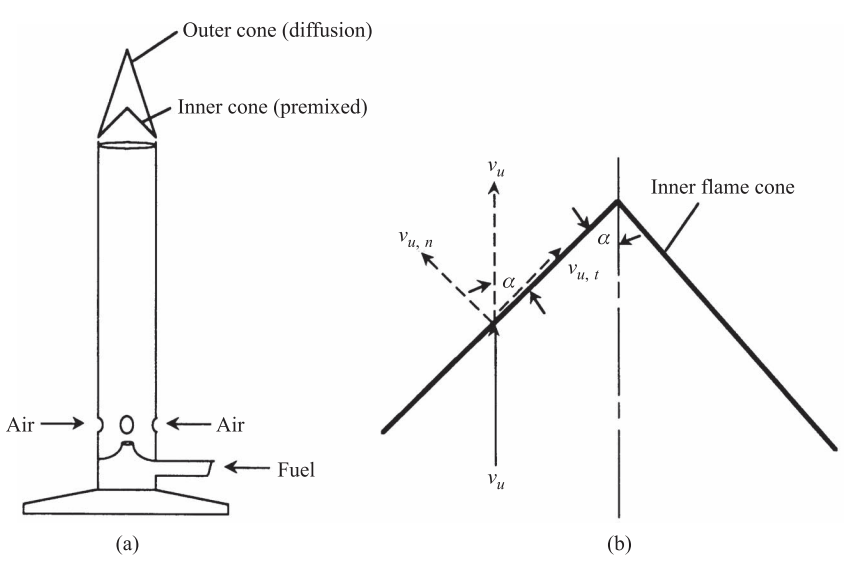
\includegraphics[width=.32\textwidth]{img/bunsen.png}
\end{figure}
由于火焰传播速度和未燃气流速度在火焰面法线方向的分量处处相等:
\begin{equation}
    S_\mathrm{L} = v_\mathrm{u}\sin \alpha
\end{equation}

\subsection{简化分析}
\subsubsection{假设}
\begin{enumerate}
    \item 一维、等面积、稳态流
    \item 忽略动能、势能,忽略黏性力做功,忽略热辐射。
    \item 忽略火焰前后的很小的压力变化,即压力是常数。
    \item 热扩散和质量扩散分别服从傅里叶定律和菲克扩散定律。假定是二元扩散。
    \item  路易斯数,\(Le = \alpha/\mathcal{D} = k/(\rho c_p \mathcal{D})\)为1。
    \item 混合物的比热容与温度及其组成无关。
    \item 燃料和氧化剂通过一步放热反应生成产物。
    \item 氧化剂等于化学当量或者过量混合,燃料完全消耗。
\end{enumerate}

\subsubsection{守恒定律}
\begin{enumerate}
    \item 质量守恒;
    \item 组分守恒,利用总包反应方程式,根据燃料的流量,分别表达燃料、氧化剂和产物三者的守恒方程;
    \item 能量方程:利用Shvab-Zeldovich形式的能量守恒方程,总和利用\(Le=1.0\)的假设,得到方程。
\end{enumerate}

\subsubsection{求解}
假定温度是\_/\(^-\)的形式,即温度在很小的距离\(\delta\)内,从低温到了高温,定义这个距离为火焰厚度。后面就代入到方程里面开始积分吧。主要处理的方程就是:
\begin{equation}
    {\dot{m}}^{\prime\prime}{\frac{\mathrm{d}T}{\mathrm{d}x}}-{\frac{1}{c_{p}}}{\frac{\mathrm{d}\left(k{\frac{\mathrm{d}T}{\mathrm{d}x}}\right)}{\mathrm{d}x}}=-{\frac{{\dot{m}}_{F}^{\prime\prime\prime}\Delta h_{c}}{c_{p}}}.
\end{equation}
一共积分两次,一次从\(-\infty\to\infty\),一次从\(-\infty\to\delta/2\)

定义平均反应速度为:

\begin{equation}
    \overline{\dot{m}}_\mathrm{F}''' = \frac{1}{T_\mathrm{b} - T_\mathrm{u}}\int_{T_\mathrm{u}}^{T_\mathrm{b}}\dot{m}_F'''\dd T
\end{equation}
实际计算的时候,也采用下面的方法:
\begin{equation}
    \overline{\dot{m}}_F''' = \overline{\dot{\omega}}_F MW_\mathrm{F}
\end{equation}
计算\(\overline{\dot{\omega}}_F\)的时候,用平均的温度和浓度就好。

注意,由于我们在推导的过程中是在\(-\infty\to \delta/2\)这一区间上进行积分的,其中包含了一个假设就是认为\(\dot{m}_\mathrm{F}'''\)等于0,所以我们在计算平均温度时:
\begin{equation}
    \overline{T} = \frac{1}{2}\left[\frac{1}{2}(T_\mathrm{b} + T_\mathrm{u})+T_\mathrm{b}\right]
\end{equation}

最后的结果是:
\begin{equation}
    S_\mathrm{L} = \left[-2\alpha (\nu+1)\frac{\overline{\dot{m}}'''_\mathrm{F}}{\rho_\mathrm{u}}\right]^{1/2}
\end{equation}

\begin{equation}
    \delta = \left[\frac{-2\rho_\mathrm{u}\alpha}{(\nu+1)\overline{\dot{m}}_F'''}\right]^{1/2}
\end{equation}
或者也可以写作:
\begin{equation}
    \delta = 2\alpha/S_L
\end{equation}

\subsection{详细分析}
\subsection{影响火焰速度和厚度的因素}
\begin{enumerate}
    \item 过量空气系数:稍稍缺氧时\((phi>1)\),火焰传播速度最大,那个时候往往火焰厚度最薄;
    \item 燃料化学结构;
    \begin{enumerate}
        \item 烷烃最大火焰传播速度为(0.7 m/s),几乎与烷烃的碳数无关;
        \item 非饱和碳氢化合物,碳原子少的火焰传播速度大;
        \item 但是碳原子多到一定程度也就基本不下降了。
    \end{enumerate}
    \item 未燃气体温度:提高未燃气体温度可以大大促进化学反应速度,从而增大\(S_L\)的值;
    \item 压力的影响:不是说\(n\)等于2的时候就没有影响了,实际上,这个时候时成反比;
    \[{\cal S}_{L}\propto\overline{{{T}}}^{0.375}T_{u}T_{b}^{-n/2}\exp(-E_{A}/2R_{u}T_{b})P^{(n-2)/2}\]
\end{enumerate}

\subsection{选定燃料的火焰传播速度计算式}
Metghalhi-Kech关系式:
\begin{equation}
    S_\mathrm{L} = S_\mathrm{L,ref}\left(\frac{T_\mathrm{u}}{T_\mathrm{u,ref}}\right)^\gamma\left(\frac{P}{P_\mathrm{ref}}\right)^\beta (1-2.1 Y_\mathrm{dil})
\end{equation}
具体细节可以看237页。

\subsection{熄火、可燃性、点火}

\subsubsection{冷壁熄火}
\textbf{点火和熄火准则}:
\begin{enumerate}
    \item 仅当足够多的能量加入到可燃气体中,使和稳定传播的层流火焰一样厚的一层气体的\textbf{温度升高到绝热燃烧温度},才能点燃。
    \item 板形区域内化学反应的放热速率必需近似平衡于由于热传导从这个区域散热的速率。
\end{enumerate}

考虑一个间距为\(d\)的平行板,研究它的熄火问题。热量流失依靠导热:
\begin{equation}
    \left|\frac{\dd T}{\dd x}\right| = \frac{T_\mathrm{b} - T_\mathrm{w}}{d/b}
\end{equation}

这里的\(b\)显然是一个至少比2大的数字,而且实际上大不少。后面经过数学上的一番倒腾,可以得到:
\begin{equation}
    d = \sqrt{b}\delta
\end{equation}

不难发现,熄火距离是要比火焰厚度要大的。

\subsubsection{可燃极限}

\textbf{可燃下限}是允许稳态火焰传播的燃料含量最低的混合气体(\(\Phi<1\)),而\textbf{可燃上限}则指允许火焰传播的燃料含量最高的混合气体(\(\Phi>1\))。

\subsubsection{点火}

着火分类:
\begin{enumerate}
    \item 化学自燃:不需外界加热,靠自身化学反应就可着火;
    \item 热自燃:混合气加热到一定温度在整个容积中着火。
\end{enumerate}

\textbf{简化的点火分析}:
\begin{itemize}
    \item 确定临界半径;
    \item 确定最小点火能量。
\end{itemize}

这里也是利用傅立叶导热定律进行分析,结论是:
\begin{eqnarray}
    R_\mathrm{crit}&=& (\sqrt{6}/2)\delta\\
    E_{\mathrm{ign}}&=&61.6P\left(\frac{c_{p}}{R_{b}}\right)\left(\frac{T_{b}-T_{u}}{T_{b}}\right)\left(\frac{\alpha}{S_{L}}\right)^{3},
\end{eqnarray}其中\(R_b = R_u/MW_b\)。

\textbf{压力、温度和当量比的影响}
\begin{equation}
    E_\mathrm{ign}\propto P^{-2}
\end{equation}
增大压力或者初始温度,最小点火能量都会降低。

\subsubsection{火焰稳定}
\textbf{回火}:火焰进入燃烧器和喷口内继续传播而不熄灭;发生在燃料气流减小或关闭时。危害:损坏燃烧设备,甚至爆炸。回火通常是瞬态的,发生在燃料气流减小或关闭时。局部火焰传播速度超过局部气流速度。当燃料气流停止时,火焰就会通过任何比熄火距离大的管子或喷口而发生回火。所以说火焰传播速度大的燃料比较容易发生回火,In comparison with 人工煤气 and 甲烷,后者回火稳定性更加好。

\textbf{推举}:火焰与燃烧器管子或喷口不接触,而是稳定在离喷口一定距离的位置;容易形成未燃气体逃逸。


\section{层流扩散火焰}

\subsection{概述}
\subsection{无反应的恒定密度层流射流}
\subsubsection{物理描述}
无限大的容器里面充满着静止的流体(氧化剂),一股无反应的流体(燃料)喷入。

\textbf{气流核心}: 黏性力和扩散还不起作用,流体的速度和射流流体的质量分数保持不变,等于喷嘴出口的值。{\tiny 如果这个情况在管内流动那就完全不同了,根据质量守恒,显然它会加速。}

\begin{figure}[H]
    \centering
    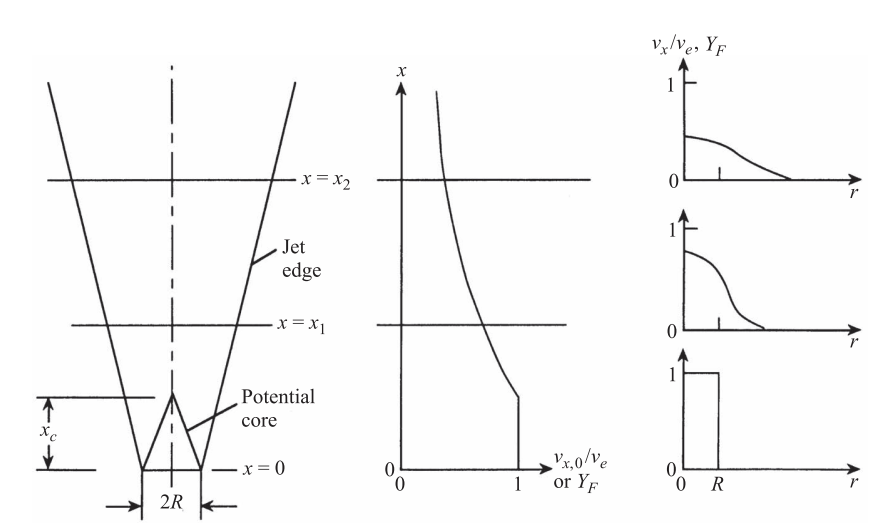
\includegraphics[width=.3\textwidth]{img/laminar_jet.png}
\end{figure}

显然存在着两个守恒:动量守恒和质量守恒,
\begin{eqnarray}
    2\pi\int_0^\infty \rho(r,x)v_x^2(r,x)r\dd r &=& \rho_e v_e^2\pi R^2\\
    2\pi\int_0^\infty \rho(r,x)v_x(r,x)Y_F(r,x)r\dd r &=& \rho_e v_e \pi R^2 Y_{F,e}
\end{eqnarray}

\subsubsection{假设}
\begin{enumerate}
    \item 射流和周围流体的摩尔质量相等。基于理想气体的性质,可以认为压力和温度都是常数,即整个流场内流体的密度为常数。
    \item 菲克扩散定律的简单二元扩散。
    \item 动量和组份扩散率为常数且相等等于1,施密特数(\(Sc\equiv \nu/\mathcal{D}\)等于1。
    \item 只考虑径向的动量和组分扩散,忽略轴向扩散。由于出口处轴向扩散很重要,所以下面的分析不适用于那里。
\end{enumerate}

\subsubsection{守恒定律}

\begin{equation}
    \begin{aligned}
        &\text{Mass:}&\frac{\pp v_x}{\pp x}+\frac{1}{r}\frac{\pp(v,r)}{\pp r}&=0\\
        &\text{Axial momentum:}& v_x \frac{\pp v_x}{\pp x}+ v_r\frac{\pp v_x}{\pp r} &= v\frac{1}{r}\frac{\pp}{\pp r}\left(r\frac{\pp v_x}{\pp r}\right)\\
        &\text{Species:}& v_x \frac{\pp Y_F}{\pp x} + v_r \frac{\pp Y_F}{\pp r}&=\mathcal{D}\frac{1}{r}\frac{\pp}{\pp r}\left(r\frac{\pp Y_F}{\pp r}\right)
    \end{aligned}
\end{equation}

那么对于氧化剂,有:
\begin{equation}
    Y_{Ox} = 1-Y_F
\end{equation}

\subsubsection{边界条件}
\begin{enumerate}
    \item 中心线的径向速度为0;
    \[v_r(0, x)=0\]
    \item 中心线的轴向速度在水平方向上变化率为0;
    \[\frac{\pp v_x}{\pp r}(0, x)=0\]
    \item 中心线的燃料质量分数在水平方向上变化率为0;
    \[\frac{\pp Y_F}{\pp r}(0, x)=0\]
    \item 轴向速度在径向的无穷远处为0;
    \[v_x(\infty, x)=0\]
    \item 燃料质量分数在径向无穷远处为0;
    \[Y_F(\infty, x) = 0\]
    \item 在出口处,速度和燃料质量分数都均匀且相等,出口外侧都为0;
    \[
        \begin{aligned}
            v_x(r\le R, 0) &=& v_e, \\
            v_x(r>R, 0) &=&0,\\
            Y_F(r\le R, 0)&=& Y_{F,e} = 1,\\
            Y_F(r>R, 0)&=&0.
        \end{aligned}
    \]
\end{enumerate}

\subsubsection{求解}
利用相似理论来进行求解,定义包含了\(r/x\)的相似变量\(\xi\)为:
\begin{equation}
    \xi = \left(\frac{3\rho_e J_e}{16\pi}\right)^{1/2}\frac{1}{\mu}\frac{r}{x}
\end{equation}

再定义初始流体动量为:
\begin{equation}
    J_e = \rho_e v_e^2\pi R^2
\end{equation}

轴向和径向速度可以表示为:
\begin{eqnarray}
    v_x &=&\frac{3}{8\pi}\frac{J_e}{\mu x}\left[1+\frac{\xi^2}{4}\right]^2\\
    v_r &=& \left(\frac{3 J_e}{16\pi\rho_e}\right)^{1/2}\frac{1}{x}\frac{\xi-\xi^3/4}{\left(1+\frac{\xi^2}{4}\right)^2}
\end{eqnarray}

我们还可以把轴向的速度写成无量纲的形式:
\begin{equation}
    v_x/v_e = 0.375(\rho_e v_e R/\mu)(x/R)^{-1}[1+\xi^2/4]^{-2}
\end{equation}
那么对于中心线的速度,代入\(\xi=0\),可以得到:
\begin{equation}
    v_{x,0}/v_e = 0.375(\rho_e v_e R/\mu)(x/R)^{-1}
\end{equation}

中间那一坨也可以写成射流雷诺数:
\begin{equation}
    Re_j \equiv \frac{\rho_e v_e R}{\mu}
\end{equation}
如前文所述,靠近喷口的地方这个式子是不合适的。

\textbf{入射流半宽}\(r_{1/2}\):在射流的某一轴向距离处,当射流速度减小到该轴向距离处中心线速度一半时的径向距离为此轴向距离处的射流半宽。
\textbf{扩张率}:射流半宽和轴向距离的比值。
\textbf{扩张角}:正切值等于扩张率的角度。
\begin{figure}[H]
    \centering
    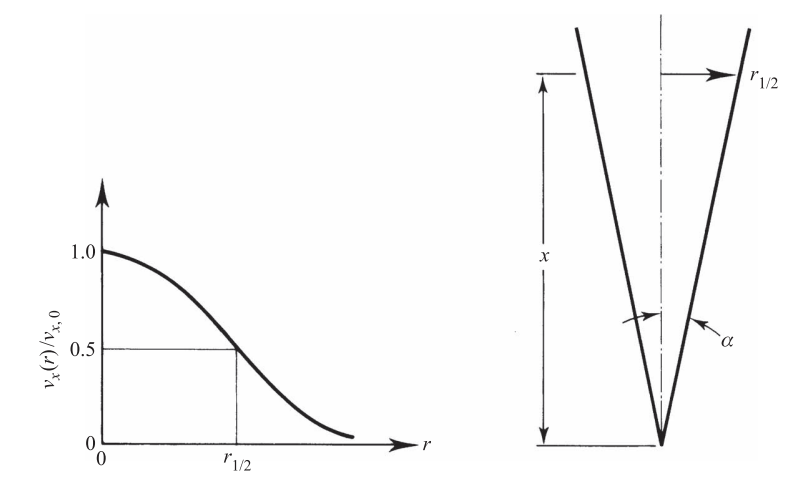
\includegraphics[width=.3\textwidth]{img/spreading_laminar.png}
\end{figure}

\begin{eqnarray}
    r_{1/2}/x &=& 2.97\left(\frac{\mu}{\rho v_e R}\right)=2.97 Re_j^{-1}\\
    \alpha &\equiv& \arctan(r_{1/2}/x)
\end{eqnarray}

对于浓度场,由于我们有施密特数等于1的假设,所以他无量纲的形式实质上和速度完全相同:
\begin{eqnarray}
    Y_F &=& 0.375 Re_j(x/R)^{-1}(1+\xi^2/4)^{-2}\\
    Y_{F,0} &=& 0.375 Re_j(x/R)^{-1}
\end{eqnarray}

上面这些式子的适用范围为:

\begin{equation}
    x/R > 0.375 Re_j
\end{equation}

\begin{enumerate}
    \item 低速射流的燃料浓度衰减到与高速射流(相差10倍)相同的值时,其轴向距离只是高速射流时的 1/10。
    \item 对于给定的燃料(\(\mu/\rho\) 为常数),燃料质量分数的空间分布只与初始的体积流量有关。
\end{enumerate}

\subsection{射流火焰的物理描述}
在流场中,燃料和氧化剂之比为化学当量的点就构成了火焰面。
对于富氧燃烧,火焰长度\(L_f\)定义为:
\begin{equation}
    \Phi(r=0, x=L_f) = 1.0
\end{equation}

\begin{itemize}
    \item 发生化学反应的区域通常是很窄的,到达顶部以前,高温区域是环状的。
    \item 按说应该考虑浮力,但是考虑到拉长之后,扩散作用也会变强,所以两个可以近似认为是抵消了。
    \item 对于圆口火焰,火焰长度和初始速度及管径都无关,粗略估算:
    \begin{equation}
        L_f\approx \frac{3}{8\pi}\frac{Q_F}{\mathcal{D}Y_\mathrm{F,stoic}}
    \end{equation}火焰长度确实是和体积流量成正比,而且还和燃料的化学当量质量分数成反比。
\end{itemize}

\subsection{简化理论描述}

\subsubsection{基本假设}


\section{液滴的蒸发和燃烧}
\subsection{概述}
\subsection{一些应用}
\subsection{液滴蒸发的简单模型}
\subsubsection{基本假设}
\begin{enumerate}
    \item 液滴在静止、无穷大的介质中蒸发。
    \item 蒸发过程是准稳态的。
    \item 燃料是单成分液体,且其气体溶解度为零。
    \item 液滴内各处温度均匀一致,并假定该温度是燃料的沸点。
    \item 路易斯数为1。
    \item 物性参数为常数。
\end{enumerate}

\subsubsection{气相分析}
这里的分析和第三章的分析是不同的,在这里,蒸发的驱动力是外在的传热,而在第三章中,驱动力主要是扩散。
\begin{enumerate}
    \item 质量守恒;
    \item 能量守恒;
    \item 液-气两相界面能量平衡:
    \[
        \dot{Q}_\text{cond}=\dot{m}(h_\text{vap}-h_\text{liq})=\dot{m}h_\text{fg}
    \]
    这里需要定义个\textit{斯波尔丁数}(\textbf{传递数})\(B\)为:
    \[
        B_q = \frac{c_{pg}(T_\infty-T_\text{boil})}{h_\text{fg}}
    \]
\end{enumerate}

\subsubsection{液滴寿命}

\begin{equation}
    \frac{\dd D^2}{\dd t} = -\frac{8 k_g}{\rho_l c_{pg}}\ln(B_q + 1)
\end{equation}

定义蒸发常数\(K\)为:
\begin{equation}
    K = \frac{8 k_g}{\rho_l c_{pg}}\ln(B_q + 1)
\end{equation}

式子在形式上~\ref{equ:03_evap}是差不多的,如果考虑路易斯数等于1,传热传质效果一样,那就完全一样了。当然,不管路易斯数是不是1,他都是需要满足\(D^2\)定律的:
\begin{equation}
    t_d=D_0^2/K
\end{equation}
这里面需要用到的物性参数近似方法为:
\begin{eqnarray}
    c_{pg} &=& c_{pF}(\overline{T})\\
    k_g &=& 0.4 k_F(\overline{T})+0.6 k_\infty(\overline{T})\\
    \overline{T}&=& (T_\mathrm{boil} + T_\infty)/2
\end{eqnarray}

\subsection{液滴燃烧的简化模型}
\subsubsection{假设}
\begin{enumerate}
    \item 环境精致,液滴之间不互相影响;
    \item 准稳态;
    \item 燃料为单组份,不会互相溶解,液气交界处存在着相平衡;
    \item 压力均匀且为常数;
    \item 气相中只有燃料蒸汽、氧化剂和燃烧产物。气相内部区域只有燃料和产物,外部区域只有氧化剂和产物;
    \item 化学当量比反应,反应无限快,火焰无限薄;
    \item 路易斯数,\(Le=\alpha/\mathcal{D}=k_g/\rho_{c,pg}\mathcal{D}\)为1;
    \item 忽略辐射;
    \item 物性参数都为常数;
    \item 液体燃料液滴是唯一的凝结相,没有碳烟和液体水存在。
\end{enumerate}

\begin{figure}[H]
    \centering
    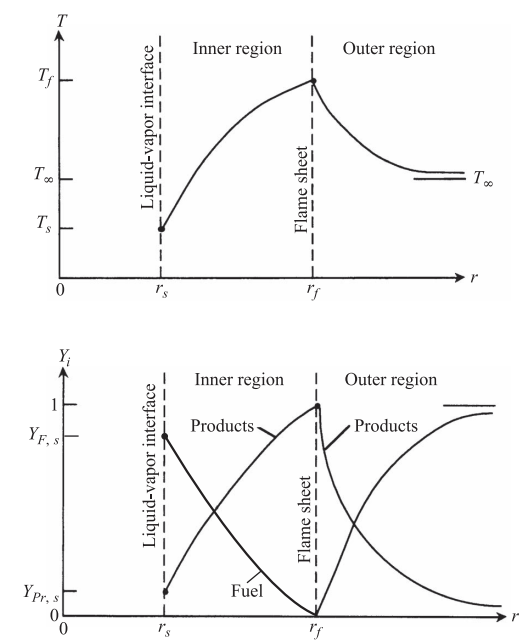
\includegraphics[width=.3\textwidth]{img/drop.png}
\end{figure}

\subsubsection{问题的表述}
求解5个未知数,求解5个关系式:
\begin{enumerate}
    \item 液滴表面的能量平衡
    \item 火焰面处的能量平衡
    \item 外区的氧化剂分布
    \item 内区的燃料蒸汽分布
    \item 液-气界面的相平衡,比如使用克劳修斯-克拉珀龙方程。
\end{enumerate}

\subsubsection{质量守恒}
总流量在任何地方都等于燃料流量.也就是燃烧速率。
\begin{equation}
    {\dot{m}}(r)={\dot{m}}_{F}=\mathrm{constant}.
\end{equation}

\subsubsection{组份守恒}
\textbf{内区}:遵守菲克定律进行扩散。
定义:
\begin{equation}
    Z_F = 1/4\pi\rho\mathcal{D}
\end{equation}

\begin{equation}
    Y_{F,s}=1-\frac{\exp(-Z_{F}\dot{m}_{F}/r_{s})}{\exp(-Z_{F}\dot{m}_{F}/r_{f})}.
\end{equation}

\textbf{外区}:交界处考虑菲克扩散定律的质量通量矢量,如果流入\(\nu\) kg的氧化剂,那么就一定会流出\(\nu+1\)kg的产物,由此我们就可以写出菲克定律,然后根据边界条件,最后解得:
\begin{equation}
    Y_{O x}(r)=\nu\left[{\frac{\exp(-Z_{F}{\dot{m}}_{F}/r)}{\exp(-Z_{F}{\dot{m}}_{F}/r_{f})}}-1\right].
\end{equation}
这里还可以得到燃烧速率和火焰半径之间的关系:

\begin{equation}
    \exp(+Z_F\dot{m}_F/r_f)  = (\nu+1)/\nu
\end{equation}

\subsubsection{能量守恒}
还是用Shvab-Zeldovich形式的能量方程,定义
\begin{equation}
    Z_T = c_{pg}/4\pi k_g
\end{equation}
\begin{enumerate}
    \item 温度分布:代入能量方程直接解酒完事儿了;
    \item 液滴表面能量平衡方程:热是从火焰通过气相导热传到液滴表面的。这些能量一部分用来蒸发燃料,其余的传到液滴内部。
    
    获得向液滴内部导热的集中方法:
    \begin{enumerate}
        \item 将液滴分为两个区,一个处于初始温度区,一个处于表面温度的表面薄层区
        \item 集总参数法;
        \item 忽略液滴的热惯性。
    \end{enumerate}
    \item 火焰面处的热量平衡:火焰处的焓变等于向液滴和无穷远处的能量传递;
    \item 液-气平衡。
\end{enumerate}

如果我们让\(T_f\to T_\infty\)以及\(r_f\to\infty\)那么这就是一个纯纯的蒸发模型,但是由于我们考虑热量传递和质量传递的影响,所以这和前面忽略这两者的简单模型是不同的。

\subsubsection{总结和求解}
定义传递数:
\begin{equation}
    B_{o,q}=\frac{\Delta h_{c}/\nu+c_{p g}\left(T_{\infty}-T_{s}\right)}{q_{i-l}+h_{f g}},
\end{equation}
燃烧速率为:
\begin{equation}
    \dot{m}_{F}=\frac{4\pi k_{g}r_{s}}{c_{p g}}\ln(1+B_{o,q}).
\end{equation}
火焰温度为:
\begin{equation}
    T_{f}=\frac{q_{i-l}+h_{f g}}{c_{p g}(1+\nu)}[{\nu}B_{o,q}-1]+T_{s}
\end{equation}
火焰半径为:
\begin{equation}
    r_{f}=r_{s}\,{\frac{\ln[1+B_{o,q}]}{\ln[(\nu+1)/\nu]}}.
\end{equation}
液滴表面的燃料质量分数为:
\begin{equation}
    Y_{F,s}=\frac{B_{o,q}-1/\nu}{B_{o,q}+1}.
\end{equation}
如果不知道液滴表面的温度,那么我们就需要结合下面的式子进行迭代求解:
\begin{equation}
    T_{s}=\frac{-B}{\ln\!\left[\frac{-Y_{F,s}P M W_{P r}}{A(Y_{F,s}M W_{F}-Y_{F,s}M W_{P r}-M W_{F})}\right]}.
\end{equation}

但是如果认为燃料已经处于沸点了,那么这个时候我们升值连\(Y_{F,s}\)的公式都可以不用,因为那个时候它等于1。

\subsubsection{燃烧速率常数和液滴寿命}

燃烧速率常数\(K\)为:

\begin{equation}
    K = \frac{8 k_g}{\rho_l c_{pg}}\ln(1+B_{o,q})
\end{equation}

在表面温度稳定不变时,这是一个常数。后面就用\(D^2\)定律就好。对于物性参数的选取:
\begin{eqnarray}
    c_{pg} &=& c_{pF} (\overline{T})\\
    k_g &=& 0.4 k_\mathrm{F}(\overline{T}) + 0.6 k_\mathrm{Ox}\\
    \rho_l&=& \rho_l(T_\mathrm{s})\\
    \overline{T} &=& 0.5(T_\mathrm{s}+T_\mathrm{f})
\end{eqnarray}

\textbf{计算差异}:采用上面的方法计算会有下面这些差异
\begin{enumerate}
    \item 实际计算的火焰温度会比一开始估计的火焰温度低好多(因为\(c_\mathrm{pg}\)不合适);
    \item 计算出来的燃烧速率还可以;
    \item 计算出来的无量纲火焰直径比实验值大很多(因为燃料蒸汽积累效应);
    \item 如果我们把环境温度设计成我们估计的火焰温度,按理说在这种纯蒸发的情况下,火焰寿命应该变长,但是实际计算出来却变短了,这是由于“理论”温度低于环境温度,如果我们把算出来的”理论“温度作为环境温度代入,这个时候算出来的纯蒸发的液滴寿命就会比燃烧的液滴寿命要更加长了。
\end{enumerate}

\subsubsection{扩展到对流条件}
\textbf{薄膜理论}的本质是将无穷远处的传热、传质边界条件用所谓的薄膜半径的边界条件替代,且其值相同。
利用\texttt{努赛尔数}\(Nu\)定义传热薄膜半径,\texttt{舍伍德数}\(Sh\)定义传质薄膜半径。
\begin{eqnarray}
    \frac{\delta_\mathrm{T}}{r_s} &=& \frac{Nu}{Nu - 2}\\
    \frac{\delta_\mathrm{M}}{r_s} &=& \frac{Sh}{Sh - 2}
\end{eqnarray}

\begin{eqnarray}
    Nu &=& \frac{h d}{k}\\
    Sh &=& \frac{h d}{\mathcal{D}}
\end{eqnarray}

\begin{figure}[H]
    \centering
    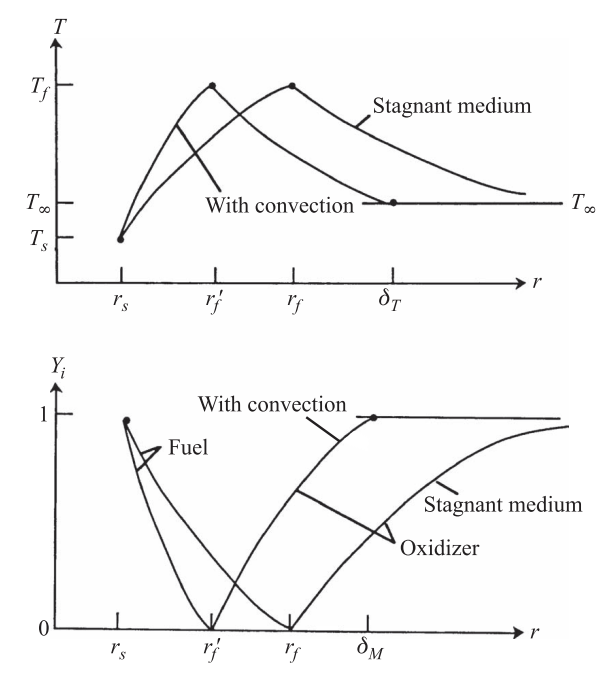
\includegraphics[width=.3\textwidth]{img/convect.png}
\end{figure}
我们相当于借此修改了边界条件的定义:
\begin{eqnarray}
    Y_\mathrm{Ox}(\delta_M) &=& 1\\
    T(\delta_T) &=& T_\infty
\end{eqnarray}

在\(Nu=2\)时,我们认为没有对流出现,在考虑路易斯数=1的情况,传热传质相同,可以得到:

\begin{equation}
    N u=2+\frac{0.557\,R e^{1/2}P r^{1/3}}{[1+1.232/(R e P r^{4/3})]^{1/2}},
\end{equation}
\begin{equation}
    \dot{m}_{F}=\frac{2\pi k_{g}r_{s}N u}{c_{p g}}\ln(1+B_{o,q}),
\end{equation}

\subsection{其他因素}
当环境温度或压力大于蒸发液体的热力学临界点时,只有用变物性才能获得守恒方程的正确表达式。


\section{湍流概论}
\subsection{概述}
\subsection{湍流的定义}
\subsection{湍流的几何尺度}
\subsubsection{4个几何尺度}
\begin{enumerate}
    \item \(L\)——\textit{流动的特征宽度}或宏观尺度:系统中最大的一个尺度,而且也是最大可能旋涡的上边界。定义平均流速下的雷诺数。
    \item \(\mathcal{l}_0\)——\textit{湍流的积分尺度}或宏观尺度:大旋涡的平均尺寸,这些涡的频率低、波长大。和\(L\)的数量级相同。可以看成是流体中脉动速度不再相关的两点间的距离。
    \item \(\mathcal{l}_\lambda\)——\textit{泰勒微尺度}:这一尺度与平均应变率有关,数量级在\(\mathcal{l}_0\)和\(\mathcal{l}_\mathrm{K}\)之间。它是黏性耗散开始影响漩涡的长度尺度。
    \item \(\mathcal{l}_\mathrm{K}\)——\textit{柯尔莫哥洛夫(Kolmogorov)微尺度}:代表了湍流动能耗散为流体内能的尺度。
\end{enumerate}
\section{湍流预混火焰}
\subsection{概述}
\subsection{一些应用}
\subsubsection{电火花点火发动机}
\subsubsection{燃气轮机}
\subsubsection{工业气体燃烧器}
\subsection{湍流火焰传播速度定义}
\begin{equation}
    S_\mathrm{t} = \frac{\dot{m}}{\overline{A} \rho_u}
\end{equation}其中\(\dot{m}\)是反应物的质量流量;\(\rho_\mathrm{u}\)是未燃气体密度;\(\overline{A}\)是时间平滑后的火焰面积。这一速度也被称为\textbf{通用消耗速度}。
\subsection{湍流预混火焰结构}
\subsubsection{实验观察}
\begin{figure}[H]
    \centering
    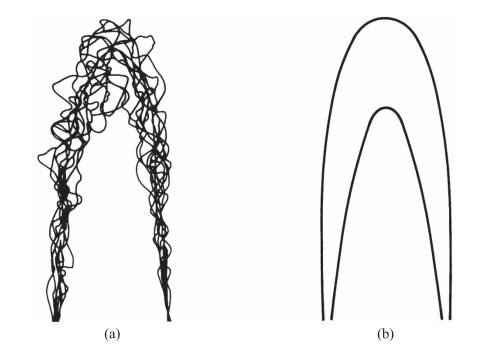
\includegraphics[width=.3\textwidth]{img/turb_prem_image.png}
\end{figure}
我们称这一有明显厚度的反应区为\textbf{湍流火焰刷}。瞬时的图像说明,实际的反应区像层流预混火焰一样,相对是很薄的。这些反应区有时也称为\textbf{层流火焰片}。

\subsubsection{三种火焰模式}

\begin{itemize}
    \item 褶皱层流火焰模式:\(\delta_L\le \mathcal{l}_\mathrm{K}\):威廉斯-克里莫夫(Williams-Klimov)判据。
    \item 分布反应模式:反应区内的输运现象就不仅受分子运动的控制,同时也受湍流运动的控制,或者至少要受湍流运动的影响。\(\delta_L > \mathcal{l}_0\):丹姆克尔(DamkGhler)判据。
    \item 漩涡小火焰模式:\(\mathcal{l}_0 > \delta_\mathrm{L} > \mathcal{l}_\mathrm{K}\)。
\end{itemize}

利用\(\mathcal{l}_\mathrm{K}\delta_\mathrm{L}\)和\(\mathcal{l}_0/\delta_\mathrm{L}\),湍流雷诺数\(Re_{t_0}\)和丹姆克尔数\(Da\),来进行分析。
\section{湍流非预混火焰}
\subsection{概述}
涉及任何一种燃烧设备,需要考虑的最终要的几个问题:

\begin{enumerate}
    \item 火焰形状和尺寸;
    \item 火焰维持与稳定;
    \item 传热;
    \item 污染排放。
\end{enumerate}

\subsection{射流火焰}
\subsubsection{总论}

\textbf{\textit{初始射流直径}和\textit{燃烧速率}对\textit{火焰尺寸}的影响}:

\begin{figure}[H]
    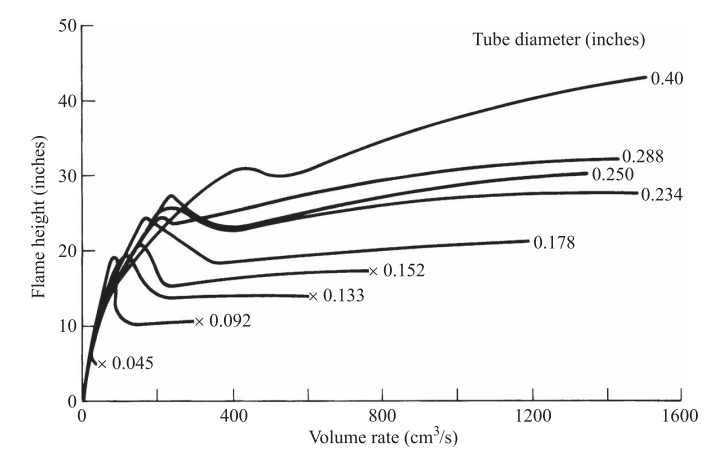
\includegraphics[width=.3\textwidth]{img/q_v_vs_h.png}
\end{figure}

\begin{enumerate}
    \item 流率小、火焰为层流时:火焰高度与初始射流直径无关,只与流率有关;
    \item 当流率增加时,湍流逐渐始影响火焰高度,出现过渡区;
    \item 在过渡区的最后,随着流率的增加,湍流程度不断增加,最后在曲线的极小值点形成比初始层流火焰要短得多的完全湍流火焰;
    \item 当流速进一步增加,火焰高度可能维持不变、也可能不断增加但斜率越来越小,增加的原因是随着燃料流率增加夹带进的空气量和混合速率也会近似成比例增加;
    \item 湍流时火焰高度明显受到初始射流直径的影响。
\end{enumerate}

\begin{multicols}{2}
    \tiny
    \begin{itemize}
        \item \textbf{附着火焰}:在足够低的流速下,火焰根部与燃烧器管子的出口非常接近(只有几个毫米);
        \item \textbf{推举火焰}:当燃料流率增加时,在火焰底部开始形成孔隙,当进一步增大流率时,会形成越来越多的孔隙,直到燃烧器喷口上没有连续的火焰;
        \item \textbf{推举距离}:管子出口与火焰根部之间的距离;
        \item 推举和吹熄。
    \end{itemize}
    
    \textbf{火焰稳定性}:
    \begin{itemize}
        \item 避免推举火焰的产生:可以用火花或者小火焰引燃进行准确的点火并保证火焰位置。但在某些应用条件下,可能需要形成一定的推举量以避免关键的燃烧器部件过热。
        \item 避免接近吹熄极限操作:在接近极限的情况下向很大的炉膛充入空燃混合物是非常危险的,一旦无法及时点燃,混合物在炉内淤积,很可能达到爆炸极限而突然爆炸,造成危险。
    \end{itemize}
\end{multicols}

\subsubsection{简化分析}
\textbf{与冷态射流的对比}
\begin{enumerate}
    \item 在速度和坐标都无量纲化之后,速度场方程时普适的;
    \item 射流扩张角时常数,与射流出口速度和直径无关;
    \item 漩涡年度与流场位置无关,正比于喷嘴出口速度和直径。
\end{enumerate}

当然燃烧后就不能像层流非预混一样和冷态射流那么相似了。浮力的作用使得射流火焰与等温射流之间的相似不再适用这也正好可以解释对于更大直径的喷管,湍流阶段的火焰长度将不恒定。

\textbf{守恒标量回顾}:

守恒标量-混合物分数\(f\)
\begin{eqnarray}
    f &=& \frac{\phi}{(A/F)_\mathrm{stoic}+\phi} \\
    f_s &=& \frac{1}{(A/F)_\mathrm{stoic}+1} \\
    \phi &=& \frac{(A/F)_\mathrm{stoic}}{(A/F)}
\end{eqnarray}

\(f\)的重要特性:
\begin{enumerate}
    \item 火焰边界处的\(f\)值\(f_s\)用来定义火焰边界;
    \item \(f\)只与\(\phi\)有关;
    \item 方程没有源项,\(f\)在整个流场中保持守恒。
\end{enumerate}

\textbf{假设}:还有一些细节可以翻翻书。

\begin{multicols}{2}
    \tiny
    \begin{enumerate}
        \item 稳态、轴对称的时均流场,即燃料由半径为R的圆管射出,在静止、无限大的空气中燃烧。
        \item 与湍流输运相比,动量、组分和能量的分子输运相对不重要。
        \item 湍流动量扩散系数,即旋涡黏度,在整个流场中守恒,且\(\epsilon=0.0285 v_e R\)。通过忽略密度的脉动,将11章提出的恒密度射流的混合长度假设扩展到变密度反应射流。
        \item 忽略所有关于密度脉动的相关项。
        \item 动量、组分和能量的湍流输运都相等:施密特数\(\nu/\mathcal{D}\)、普朗特数\(\nu/\alpha\)和路易斯数\(\alpha/\mathcal{D}\)都相等。
        \item 忽略浮力。
        \item 忽略辐射传热。
        \item 只考虑径向的动量、组分和能量的湍流扩散,忽略轴向的。
        \item 喷嘴出口处燃料射流速度相同,即帽式分布。
        \item 混合物性质由燃料(假想燃料)、氧化剂和产物三种组分决定。
        \item 在采用状态关系式确定平均密度时,忽略混合物分数的脉动。
    \end{enumerate}
\end{multicols}

\textbf{守恒定律的应用}
湍流雷诺数的定义:
\begin{equation}
    Re_T \equiv \frac{v_e R}{\epsilon}
\end{equation}

根据假设10和假设11,温度的状态参数式是\(\overline{f}\)的简单分段线性方程:
\begin{figure}[H]
    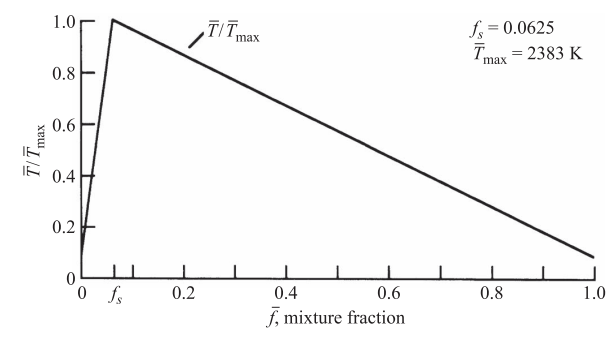
\includegraphics[width=.3\textwidth]{img/f_vs_t.png}
\end{figure}

\textbf{模型解}

\begin{enumerate}
    \item 火焰的高度是喷嘴直径的45倍;
    \item 长宽比(火焰高度和宽度的比值)约11:1,该值比用碳氢射流火焰实验测定的7:1要大一些。
    \item 尽管对湍流射流火焰模型作了大量简化,火焰的总体特征还是能够得到良好的预测,只是精度差些。忽略密度脉动的变化可能对计算准确性影响最大。
\end{enumerate}

\subsubsection{火焰长度}
火焰的可视长度要大于靠温度或浓度测量所得出的长度。

\textbf{影响火焰长度的因素}
\begin{enumerate}
    \item 火焰中射流初始动量与作用在火焰上浮力的比:\(Fr_t\);
    \item 化学当量值\(f_s\);
    \item 射流密度与环境气体密度的比\(\rho_e/\rho_\infty\);
    \item 初始射流直径\(d_j\)。
\end{enumerate}

湍流射流火焰弗劳德数\(Fr_f\)的定义:
\begin{equation}
    Fr_f = \frac{v_e f_s^{3/2}}{{\left(\frac{\rho_e}{\rho_\infty}\right)}^{1/4}{\left[\frac{\Delta T_f}{T_\infty}g d_j\right]}^{1/2}}
\end{equation}
其中\(\Delta T_f = T_f - T_\infty\),表示因燃烧产生的特征温升。
\begin{itemize}
    \item \(Fr_f\)很小,火焰受浮力控制;
    \item \(Fr_f\)很大,初始射流动量决定混合及火焰中的速度场。
\end{itemize}
\textbf{浮力对射流火焰的影响}:
\begin{figure}[H]
    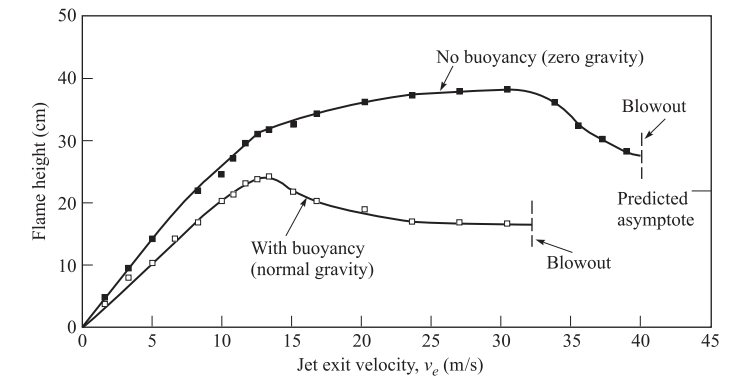
\includegraphics[width=.3\textwidth]{img/buoyancy.png}
\end{figure}
\begin{itemize}
    \item 由于浮力引起的流动,增强了火焰中各成分混合,导致火焰长度比无浮力情况下的长度要短很多;
    \item 如果火焰一直没有吹熄现象发生,随着射流速度的增加,火焰长度最终接近同一渐近值。
\end{itemize}

\textbf{当量值}:\(f_s\)比较小的燃料需要更多的空气才能达到燃烧的化学当量;\(f_s\)越小,火焰越长;丙烷需要的当量空气质量是一氧化碳的6倍,所以丙烷火焰的长度大概是一氧化碳火焰长度的7倍。

\textbf{动量直径}组合了第三和第四个因素的影响:
\begin{equation}
    d_j^* = d_j(\rho_e/\rho_\infty)^{0.5}
\end{equation}

\textbf{关联性}
\begin{figure}[H]
    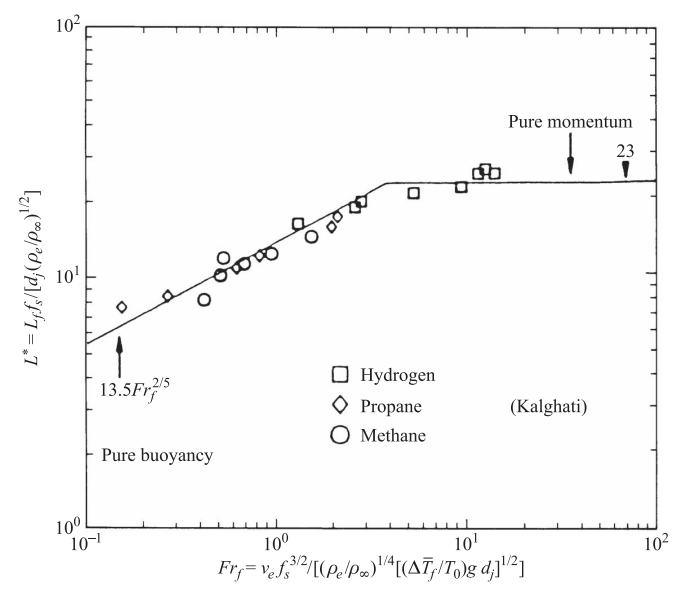
\includegraphics[width=.3\textwidth]{img/fr.png}
\end{figure}
无量纲火焰长度:
\begin{equation}
    L^* = \frac{L_f f_s}{d_j (\rho_e/\rho_\infty)^{0.5}}
\end{equation}

\begin{enumerate}
    \item 浮力控制:
    \begin{equation}
        L^* = \frac{13.5 Fr_f^{0.4}}{(1+0.07 Fr_f^2)^{0.2}}, \quad Fr_f < 5.0
    \end{equation}
    \item 动量控制:
    \begin{equation}
        L^* = 23, \quad Fr_f\ge 5.0
    \end{equation}
\end{enumerate}

\subsubsection{火焰辐射}
\textbf{辐射分数}\(\chi_R\):
\begin{equation}
    \chi_R = \frac{\dot{Q}_\mathrm{rad}}{\dot{m}_\mathrm{F}\Delta h_c}
\end{equation}
其中\(\dot{m}_F\)是供给燃料的质量流率;\(\Delta h_c\)是燃料的热值

\begin{enumerate}
    \item 燃料的辐射分数与发烟点相对应;
    \item 辐射分数的大小由火焰尺寸和释热率决定:当固定燃烧速率而减小火焰尺寸,或固定火焰尺寸而增大燃烧速率时,都会使辐射分数 减小。    
\end{enumerate}

\subsubsection{推举和吹熄}

有三种理论可以解释推举火焰:
\begin{enumerate}
    \item 层流火焰速度最大处的局部气流速度恰好与湍流预混火焰的燃烧速度相等:\(\overline{v}(S_{L,\max})=S_T\);
    \item 流场局部的应变速率超过了层流扩散火焰面的临界熄火应变速率:\(\epsilon>\epsilon_{crit}\);
    \item 大尺度流场结构中高温产物与未燃混合物的有效返混时间小于点火的临界化学反应时间:\(\tau_\mathrm{local-mixing}<\tau_\mathrm{chem,crit}\)。
\end{enumerate}

\begin{enumerate}
    \item 推举高度与烧嘴直径之间没有多少相关性;
    \item 层流火焰速度越大,推举高度h曲线增加的斜率越大。
\end{enumerate}

\textbf{火焰吹熄的原因}:当流速增加时,推举高度不断上升。火焰根部的流速和湍流燃烧速度都随推举距离的增加而减小。在某个临界点之后,湍流燃烧速度的减小速率>局部流速的减小速率(最大层流燃烧速度处),再也找不到可以平衡的点,两者差距越来越大,发生吹熄。


有关系式可以计算射流火焰吹熄速度,具体可以看416页。当燃料固定,吹熄速度将随射流直径的增加而增加。这也就是为什么油井熄火十分困难的原因(通常油井直径比较大)。

\subsection{其他结构下的非预混火焰}
应用旋流主要有两个原因:第一,当旋流足够大时,可以产生回流区来稳定火焰;第二,旋流的程度还可以控制火焰的长度。

旋流数\(S\)的定义:\(S=M/(I r_0)\),其中\(M\)是切向动量矩,\(I\)是轴向动量,\(r_0\)为特征尺寸。当\(S\ge 0.6\)时为强旋流。

旋流火焰的作用:
\begin{enumerate}
    \item 稳定火焰:
    \item 控制火焰长度:旋流大大加强了空气与燃料的混合。
\end{enumerate}
\section{固体的燃烧}
\subsection{概述}
\subsection{燃煤锅炉}
\subsection{非均相反应}
\begin{enumerate}
    \item 反应物分子通过对流和(或)扩散作用到达固体表面;
    \item 反应物分子在固体表面被吸附;
    \item 包含被吸附分子、固体表面自身及气相分子的多种化合作用的基元反应;
    \item 产物分子在固体表面的解吸附;
    \item 产物分子通过对流和(或)扩散作用离开固体表面。
\end{enumerate}
三种反应模式:
\begin{enumerate}
    \item 如果反应物分子A的吸附能力较弱:\(\mathcal{R}=k(T)[\mathrm{A}]\);
    \item 如果A强吸附:\(\mathcal{R}=k(T)\);
    \item 如果A弱吸附、B强吸附:\(\mathcal{R}=k(T)\frac{[\mathrm{A}]}{[\mathrm{B}]}\)。
\end{enumerate}

\subsection{碳的燃烧}
\subsubsection{概述}
碳反应的总包反应,Power-law:
\begin{eqnarray}
    \mathrm{C + O_2} &\overset{k_1}{\rightarrow}& \mathrm{CO_2}\\
    \mathrm{2C + O_2} &\overset{k_1}{\rightarrow}& \mathrm{2CO}\\
    \mathrm{C+CO_2} &\overset{k_1}{\rightarrow}& \mathrm{2CO}\\
    \mathrm{C+H_2O} &\overset{k_1}{\rightarrow}& \mathrm{CO+H_2}
\end{eqnarray}

反应生成的主要产物CO扩散出去之后燃烧产生\(\mathrm{CO_2}\)。

在一定的条件下,颗粒内部扩散在碳的燃烧中发挥着重要的作用。但是在下面的分析中假定扩散无法通过固体表面。

\subsection{单模模型}
\textbf{假设}:
\begin{enumerate}
    \item 燃烧过程为准稳态;
    \item 球形碳颗粒在无限大的、静态的环境中燃烧;
    \item 在碳颗粒表面,碳与化学当量的氧气反应,产生二氧化碳;
    \item 气相仅由氧气、二氧化碳和惰性气体组成;
    \item \(k,c_p,\rho\mathcal{D}\)都为常数,路易斯数为1;
    \item 颗粒内部扩散可被忽略;
    \item 碳颗粒温度均匀,以灰体形式和外界环境辐射换热,而且没有中间介质的参与。
\end{enumerate}

\textbf{问题描述}:
求出碳的质量燃烧速率\(\dot{m}_C\)、表面温度\(T_s\)。这边只考虑组份及能量平衡方程。

\textbf{总的质量和组分守恒}:

流出去的质量流率恰好等于碳的燃烧速率。
\begin{eqnarray}
    \mathrm{1~kgC} + \nu_1 \mathrm{kg O_2}&\rightarrow& (\nu_1+1)\mathrm{kgCO_2}\\
    \nu_\mathrm{I} &=& \frac{21.999\mathrm{kgO_2}}{12.01\mathrm{kg}\mathrm{C}} = 2.664.
\end{eqnarray}
\begin{multicols}{2}
    \tiny
    \begin{figure}[H]
        \centering
        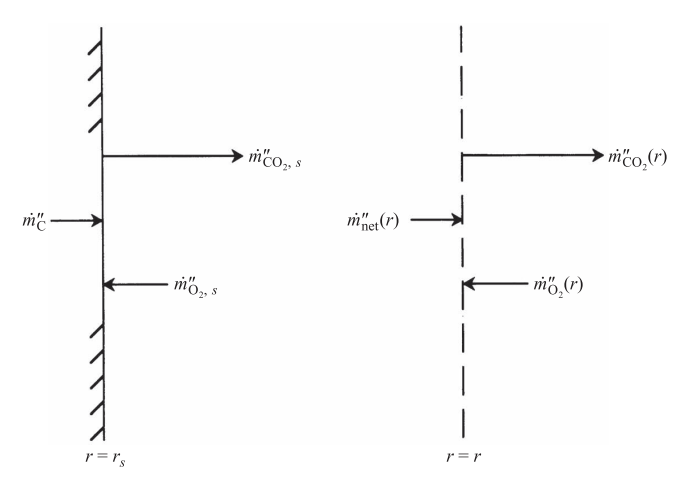
\includegraphics[width=.15\textwidth]{img/mass_flux_carbon.png}
    \end{figure}
    \begin{eqnarray}
        \dot{m}_\mathrm{O_2} &=& \nu_\mathrm{I} \dot{m}_\mathrm{C}\\
        \dot{m}_\mathrm{CO_2} &=& (\nu_\mathrm{I} + 1) \dot{m}_\mathrm{C}
    \end{eqnarray}
    然后在均匀相当中就可以运用菲克定律了。后面就是一通算。最后可以得到碳的通量:
\end{multicols}

\begin{equation}
    \dot{m}_\mathrm{C} = 4\pi r_s \rho \mathcal{D} \ln\left(\frac{1+Y_\mathrm{O_2,\infty}/\nu_\mathrm{I}}{1+Y_\mathrm{O_2,s}/\nu_\mathrm{I}}\right)
\end{equation}

\textbf{表面化学动力学}:认为碳和氧气的反应时一级的,可以进行一些计算,详见436
\textbf{电路比拟}
\begin{eqnarray}
    \dot{m}_\mathrm{C} &=& \frac{Y_\mathrm{O_2,\infty}-0.0}{R_\mathrm{kin}+R_\mathrm{diff}}\\
    R_\mathrm{kin} &\equiv& 1/K_\mathrm{kin} = \frac{\nu_\mathrm{I}R_u T_s}{4\pi r_s^2 MW_\mathrm{mix}k_c P}\\
    R_\mathrm{diff} &\equiv& \frac{\nu_\mathrm{I}+Y_\mathrm{O_2, s}}{\rho \mathcal{D}4\pi r_s}
\end{eqnarray}
\textbf{碳燃烧控制情况}

\begin{enumerate}
    \item \textbf{扩散控制}:\(R_\mathrm{kin}/R_\mathrm{diff}\ll1\):\(r_s\uparrow, T_s\uparrow, P\uparrow\);
    \begin{enumerate}
        \item 在\(k_c\)很大,快速的表面反应;
        \item 根据阿仑尼乌斯,这个时候温度很高;
        \item 也可能是碳表面上氧气浓度很小,接近于0.0,导致化学动力学参数中没有一个可以影响到燃烧速率。
    \end{enumerate}
    \item \textbf{化学动力学控制}:\(R_\mathrm{kin}/R_\mathrm{diff}\gg1\):\(r_s\downarrow, T_s\downarrow, P\downarrow\)。
    \begin{enumerate}
        \item \(R_\mathrm{diff}\)很小;
        \item \(Y_\mathrm{O_2,s}\)和\(Y_\mathrm{O_2,\infty}\)基本相等,表面氧气浓度比较大;
    \end{enumerate}
\end{enumerate}
\begin{equation}
    {\frac{R_{\mathrm{kin}}}{R_{\mathrm{diff}}}}\equiv\left({\frac{\nu_{1}}{\nu_{1}+Y_\mathrm{O_{2},s}}}\right)\left({\frac{R_{u}T_{s}}{M W_{\mathrm{mix}}P}}\right)\left({\frac{\rho \mathcal{D}}{k_{c}}}\right)\left({\frac{1}{r_{s}}}\right)
\end{equation}

\textbf{能量守恒}:一通算可以得到温度的分布,具体可以看440。

\begin{figure}[H]
    \centering
    \begin{subfigure}{.15\textwidth}
        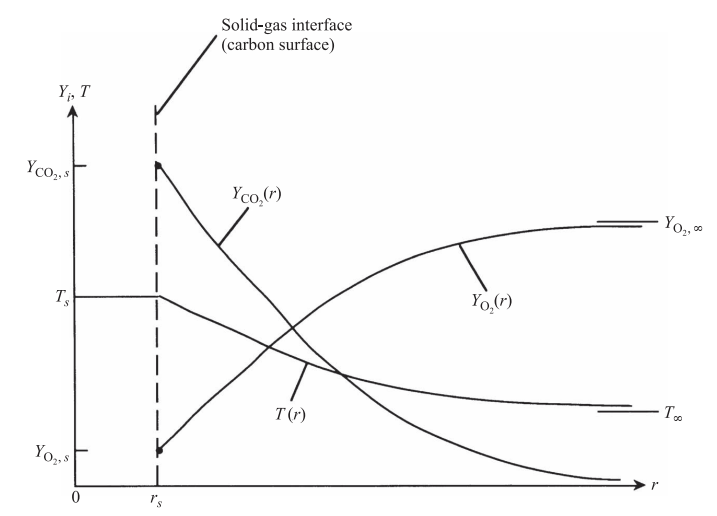
\includegraphics[width=.99\textwidth]{img/single_film.png}
        \caption{单模模型}
    \end{subfigure}
    \begin{subfigure}{.15\textwidth}
        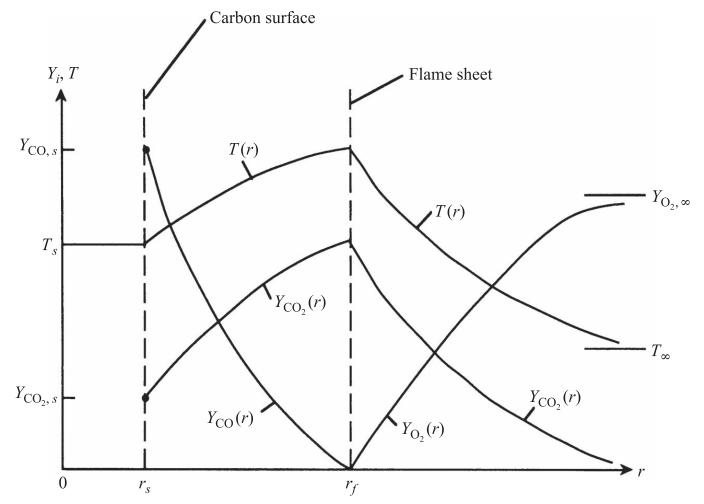
\includegraphics[width=.99\textwidth]{img/double_film.png}
        \caption{双膜模型}
    \end{subfigure}
\end{figure}

\subsubsection{双模模型}
\textbf{化学计量学}
\begin{eqnarray}
    \mathrm{1kgC}+\nu_s \mathrm{kgCO_2}&\rightarrow& (\nu_s+1)\mathrm{kgCO} \\
    \mathrm{1kgC}+\nu_f \mathrm{kg O_2} &\rightarrow& (\nu_f+1)\mathrm{kg CO_2}
\end{eqnarray}

其中
\begin{eqnarray}
    \nu_s &=& \frac{44.01}{12.01} = 3.664\\
    \nu_f &=& \nu_s - 1
\end{eqnarray}

然后我们就可以把各个组份的质量通量和碳的质量通量联系起来。

\textbf{组分守恒方程}:
应用菲克扩散定律可以获得分别描述内部区域和外部区域\(CO_\mathrm{2}\)分布的微分方程。单靠这个也不够,还需要利用化学动力学方程来对之进行封闭。

\textbf{表面化学动力学}:燃烧速率可以表达成与单膜反应中相同的形式,不过到他这儿是和二氧化碳反应生成一氧化碳。
\textbf{封闭性}

\subsubsection{碳颗粒燃烧时间}
依然是\(D^2\)定律,这里的燃烧速率:

\begin{equation}
    K_B = \frac{8\rho \mathcal{D}}{\rho_c}\ln(1+B)
\end{equation}

这里的传递数\(B\)对于单模选择\(B_\mathrm{O,m}\),对于双模选择\(B_\mathrm{CO_2, m}\)。
具体的计算可以看444页的例题。

忽略表面的化学动力学将会使燃烧速度有16.8 \%(=100\%(2.22-1.9)/1.9)的误差。表面温度(或压力)越低,动力学的影响就越大。 另外,随着燃烧的进行,\textit{颗粒直径也将不断减小,同样会使得动力学因素变得重要}。

\textbf{对流环境}:第十章的膜理论。

\subsection{煤的燃烧}
\subsubsection{煤的工业和元素分析}
\begin{figure}
    \centering
    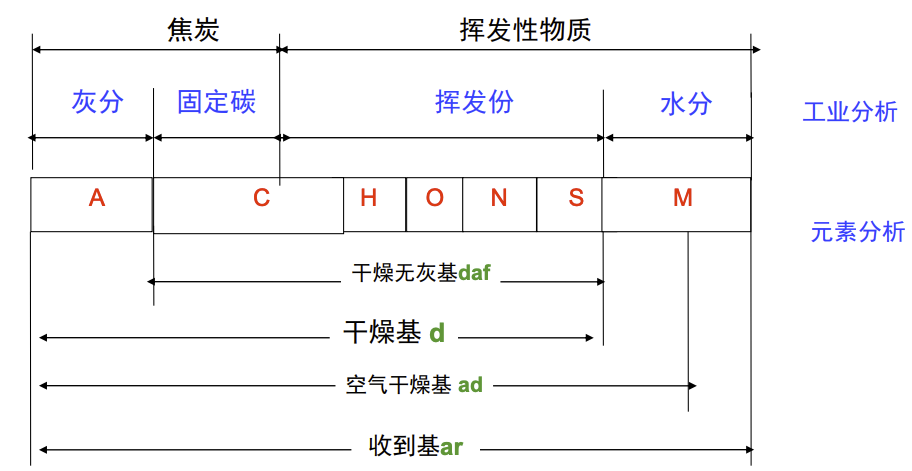
\includegraphics[width=.3\textwidth]{img/coal.png}
\end{figure}
\begin{enumerate}
    \item 收到基(应用基):以实际使用的煤为基准而测出的煤各元素的质量百分组成。
    \item 空气干燥基(分析基 ):以实验室使用的风干煤样(用温度为20\(^\circ\)C,相对湿度为70\%的空气)为基准而测出的煤各元素的质量百分组成。
    \item 干燥基:以无水的煤为基准而测出的煤各元素的质量百分组成。
    \item 干燥无灰基(可燃基 ):以无水、无灰的煤为基准而测出的煤各元素的质量百分组成。
\end{enumerate}

\subsubsection{煤的种类及特点}
\begin{enumerate}
    \item 褐煤:外观褐色,光泽黯淡。水分含量高,热值低,密度较小,含氧量高,化学反应强,极易氧化和自然。常作为加压气化燃料,锅炉燃料;
    \item 烟煤:挥发份含量高、灰分及水分较少,发热量高。可划分贫煤、焦煤、气煤。
    \item 无烟煤:挥发份含量低,燃点较高,燃烧时无粘结性。
\end{enumerate}
\section{污染物排放}
\subsection{概述}
\subsection{污染物的危害}
\begin{enumerate}
    \item 改变大气和降水的特性;
    \item 对植被有害;
    \item 污染和破坏了各种材料;
    \item 可能提高人类的发病率和死亡率。
\end{enumerate}

\subsection{排放的量化描述}
\subsubsection{排放因子}
\begin{equation}
    \mathrm{EI}_i = \frac{m_{i,\mathrm{emitted}}}{m_{\mathrm{F,burned}}}
\end{equation}
对于碳氢化合物在空气中的燃烧,排放因子可以由指定测量的组分浓度(摩尔分数)和所有含碳组分的浓度来决定。
\begin{equation}
    \mathrm{EI}_i = \left(\frac{\chi_i}{\chi_\mathrm{CO} + \chi_\mathrm{CO_2}}\right)\left(\frac{x MW_i}{MW_\mathrm{F}}\right)
\end{equation}

排放因子的测量与任何(比如)空气稀释效果无关。

\subsubsection{折算浓度}
实际应用中,通常将排放浓度折算为燃烧产物中特定含氧量下的值。目的在于排除各种稀释情况的影响,从而能够对污染物排放进行客观的比较。

\subsubsection{各种特定的排放测量}
比质量排放=污染物的质量流量/制动力。

\subsection{预混燃烧过程的排放}

\subsubsection{氮氧化物}

\begin{enumerate}
    \item 当量比为1的层流预混燃烧火焰中,压力的影响大: 低压下NO的形成由快速NO机理中的费尼莫尔(HC-N2)以及O和OH超平衡路径来控制。高压条件下(如10atm)热力型机理产生了一半以上。
    \item 富燃料层流预混火焰,当量比的影响大。随着混合物中燃料逐渐增多,快速NO机理起主导作用,当量比为1.32时形成了约95\%NO。(总的NOx也少)。
    \item 全混流反应器(完全混合的反应器)。在反应物和产物发生强烈的返混时,快速NO机理中的超平衡O和OH的反应路径控制贫燃混合物的反应;快速NO机理中的Fenimore控制化学当量下以及富燃混合物的燃烧。
\end{enumerate}

控制策略:对于热力型NO,需要很高的活化温度。
\begin{itemize}
    \item 降低峰值温度:将废气(烟气)与新鲜空气或燃料混合。废气(烟气)再循环的作用:在给定热释放量的条件下,增加燃气的比热容,降低燃烧温度。
    \item 推迟火花点火时间:较晚的点火时间可改变燃烧过程,使最高压力刚好出现在发动机的上止点, 从而降低压力和温度。但是这样会牺牲燃油经济性。
    \item 分级燃烧:当然实际不是这样的。
    \begin{enumerate}
        \item 利用富燃燃烧的高稳定性和低NOx特性完成初步过程
        \item 在贫焰燃烧阶段将产生的CO和H2完全燃烧完
    \end{enumerate}
    \item 催化后处理技术。
\end{itemize}

\subsubsection{一氧化碳}
生成机理:
\begin{enumerate}
    \item 特定的燃烧温度下CO\(_2\)的离解;
    \item 冷壁面熄火;
    \item 未燃尽燃料部分氧化过程。
\end{enumerate}

\subsubsection{未燃烃}
\begin{enumerate}
    \item 壁面熄火产生的碳氢化合物绝大多数最终都会与高温气体混合并被氧化掉,但是在缝隙的入口和里面都会产生未燃碳氢化合物,例如在活塞端环槽脊上、环形密封处、螺旋火花塞的缝隙中;
    \item 壁面上油层对燃料的吸附和解吸附;
    \item 气缸内火焰的不完全传播;
    \item 燃料高温热解及部分氧化。
\end{enumerate}

\subsubsection{催化后处理技术}
\begin{figure}[H]
    \centering
    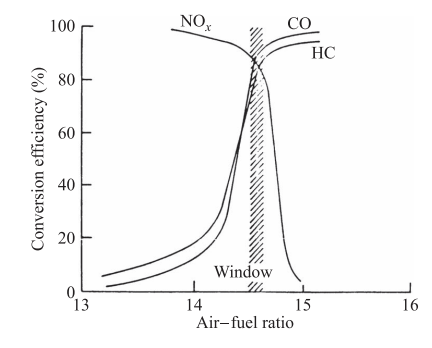
\includegraphics[width=.3\textwidth]{img/three-way.png}
\end{figure}

实际情况是不太好控制的。

\subsubsection{颗粒物}
预混燃烧,各种燃料形成碳烟的趋势不仅与燃料结构有关,还与火焰温度有关。

\subsection{非预混燃烧的排放}


\subsubsection{氮氧化物}
氮氧化物-工业燃烧设备控制策略
\begin{itemize}
    \item 低过量空气:只能有限的降低NOx排放,因为过量空气减少使CO排放增加;
    \item 分级燃烧:上游燃烧器在富燃料状态下运行,下游燃烧器只提供空气;这项技术可使NOx的减排达到10\%~40\%;
    \item 降温:在燃气工业锅炉中,用烟气再循环后, NOx的减排效果可达50\%~85\%。也可以向燃烧器中喷水来降低火焰温度。
    \item 低Nox燃烧器:还是分级燃烧的原理。
    \item 富氧燃料燃烧:加入足够大量的氧气,使氮气浓度的降低超过了燃烧温度增加的影响。
    \item 再燃:燃料总量的15\%将被直接送往贫燃区域的下游进行再燃。在再燃区内(当量比>1),NO将会和碳氢化合物及中间物质(如HCN)反应而使其降低。最后加入额外的空气,保证再燃燃料最终能燃烧完全。运用再燃技术的锅炉一般都能将NOx的排放量减小60\%。
    \item 选择性非催化还原(SNCR)-“喷氨法”。
    \item 选择性催化还原(SCR)。NOx的减排可以更大,而且操作温度更低。但是几乎是多有脱硝技术中最昂贵的,因为初期投资和运行过程中催化剂的更换成本都很高。
\end{itemize}

\subsubsection{未燃烧和一氧化碳}
\textbf{未燃碳氢化合物和CO}:

\textbf{主要途径}
\begin{enumerate}
    \item 存在过度贫燃区域难以支持快速的燃烧反应。火焰不会在过度贫燃区域内传播,在这个区域燃料发生高温热解形成部分氧化的产物,如醛类和CO。
    \item 火焰中形成过度富燃料的区域,而且没有额外的空气补充进来,或者没有足够的时间使氧化反应进行完全。
\end{enumerate}
其他途径包括:壁面熄火(柴油机)、由二次风或稀释空气的射入引起的熄火(燃气轮机)、喷管段残留燃料的滴入(柴油机)、未充分雾化的燃料液滴(燃气轮机,偶然发生)。

\textbf{颗粒物}:
燃煤产生的矿物质飞灰可以通过静电除尘等手段从尾部烟气中去除。非预混燃烧产生的主要颗粒物是碳烟。碳烟在扩散火焰的富燃区域内进行,形成的碳烟是否会从火焰中放出取决于碳烟的生成和氧化过程的平衡关系。设计燃烧系统时,使碳烟在形成前先被氧化和增加氧化速度都可以降低碳烟的排放。柴油机,燃烧后进行颗粒捕集。

\textbf{硫化物SOx}

SOx的产生:在燃烧过程中,燃料中的硫都以SO2或SO3的形式被排出,统称为SOx。控制SOx的途径:去除燃料中的硫,或去除烟气中的SOx。

\end{multicols}
\end{document}